%%%%%%%%%%%%%%%%%%%%%%%%%%%%%%%%%%%%%%%%%%%%%%%%%%%%%%%%%%%%%%%%%%%%%%%%%%%%%%%%
%2345678901234567890123456789012345678901234567890123456789012345678901234567890
%        1         2         3         4         5         6         7         8

\documentclass[letterpaper, 10 pt, conference]{Format/ieeeconf}  % Comment this line out
                                                          % if you need a4paper
%\documentclass[a4paper, 10pt, conference]{ieeeconf}      % Use this line for a4
                                                          % paper

\IEEEoverridecommandlockouts                              % This command is only
                                                          % needed if you want to
                                                          % use the \thanks command
\overrideIEEEmargins

\usepackage{amsmath,amsfonts,amssymb,mathrsfs}
\usepackage{graphicx}
\usepackage{psfrag,graphicx,epsfig,epsf}
\usepackage[ruled,linesnumbered, noend]{algorithm2e}
\usepackage{fancyhdr}
\usepackage{wrapfig}
\usepackage{subfigure}
\usepackage{mathtools}
\usepackage[permil]{overpic}
\usepackage{url}
\usepackage{color}
\usepackage{verbatim}
\usepackage{xspace}
\usepackage{cite} 
\usepackage[export]{adjustbox}

\usepackage{multirow}

\usepackage{url}
\usepackage{breakurl}
\usepackage[breaklinks]{hyperref}
\def\UrlBreaks{\do\/\do-}

\title{\LARGE \bf
%Increasing the Robustness of Packing Cubic Products:\\ Environment-aware Manipulation for a Minimalistic End-effector
Towards Robust Product Packing with a Minimalistic End-Effector
%Robust Autonomous Product Packing with a Minimalistic End-Effector  
}

% \author{TBD$^{1}$}

\author{Rahul Shome*, Wei N. Tang*, Changkyu Song,  Chaitanya Mitash, Hristiyan Kourtev,\\  Jingjin Yu, Abdeslam Boularias, and Kostas E. Bekris% <-this % stops a space
\thanks{The authors are affiliated with the Computer Science Dept. of, Rutgers University, New Brunswick, NJ, USA. email:\{jingjin.yu,abdeslam.boularias,kostas.bekris\}@cs.rutgers.edu}%
\thanks{*These authors have equally contributed to the work.}% <-this % stops a space
\thanks{The authors would like to acknowledge the support of NSF IIS:1617744 and JD-X Research and Development Center (RDC). Any opinions expressed here or findings do not reflect those of the sponsor.}}


\begin{document}



\maketitle
\thispagestyle{empty}
\pagestyle{empty}
\newcommand{\danh}[2][1=]{\todo[linecolor=blue,
			backgroundcolor=blue!5,bordercolor=black,#1]{DH:#2}}
\newcommand{\kb}[2][1=]{\todo[linecolor=green,
			backgroundcolor=green!5,bordercolor=black,#1]{KB:#2}}
\newcommand{\ks}[2][1=]{\todo[linecolor=red,
			backgroundcolor=red!5,bordercolor=black,#1]{KS:#2}}
\newcommand{\rs}[2][1=]{\todo[linecolor=orange,
			backgroundcolor=orange!10,bordercolor=black,#1]{RS:#2}}
\newcommand{\jy}[2][1=]{\todo[linecolor=black,
			backgroundcolor=black!5,bordercolor=black,#1]{JJ:#2}}

%%% Mathematical Definitions
\newcommand{\reals}{\mathbb{R}}
\newcommand{\integers}{\mathbb{Z}}

%%% Definitions for Workspace, Objects, Manipulator
\newcommand{\Wspace}{\mathcal{W}}
\newcommand{\Objects}{\mathcal{O}}
\newcommand{\Manip}{\mathcal{M}}
\newcommand{\nobj}{k}

%% Definitions for Object stuff
\newcommand{\Pspace}{\mathcal{P}}
\newcommand{\Pstable}{\mathcal{P}^s}
\newcommand{\pose}{p}
\newcommand{\GeomObj}{\mathcal{WO}}
\newcommand{\Arrange}{\mathcal{A}}
\newcommand{\Pumped}{\mathcal{A^P}}
\newcommand{\pumpedarr}{\alpha^{\mathcal{P}}}

%% Definitions for Manipulator stuff
\newcommand{\Qspace}{\mathcal{Q}}
\newcommand{\GeomManip}{\mathcal{WM}}

%% Definitions for problem and state space
\newcommand{\Tspace}{\mathbb{T}} 
\newcommand{\Xspace}{\mathbb{X}}
\newcommand{\paths}{\Pi}

%% Manipulation roadmap definition
\newcommand{\roadmap}{\mathcal{R}}
\newcommand{\graph}{\mathcal{G}}
\newcommand{\nodes}{\mathcal{V}}
\newcommand{\node}{{v}}
\newcommand{\edges}{\mathcal{E}}
\newcommand{\edge}{{e}}
\newcommand{\prmstar}{{\tt PRM$^*$}}

\newcommand{\rpg}{${\tt RPG}$}

\newcommand{\local}{\mathcal{L}}

\newcommand{\prm}{{\tt PRM}}
\newcommand{\kprmstar}{{\tt k-PRM$^*$}}
\newcommand{\rrt}{{\tt RRT}}
\newcommand{\rrtdrain}{{\tt RRT-Drain}}
\newcommand{\rrg}{{\tt RRG}}
\newcommand{\est}{{\tt EST}}
\newcommand{\rrtstar}{{\tt RRT$^*$}}
\newcommand{\srrt}{{\tt RDG}}
\newcommand{\bvp}{{\tt BVP}}
\newcommand{\rdg}{{\tt RDG}}
\newcommand{\lrg}{{\tt LRG}}
\newcommand{\alg}{{\tt ALG}}
\newcommand{\upump}{{\tt UPUMP}}
\newcommand{\prxpump}{{\tt RPG}}
\newcommand{\fixed}{{\tt Fixed}-$\alpha$-\rdg}
\newcommand{\nrob}{k}
\newcommand{\cons}{K}

\newcommand{\frnodes}{V_f}
\newcommand{\frnode}{v_f}
\newcommand{\grnodes}{V_g}
\newcommand{\grnode}{v_g}
\newcommand{\fredges}{E_f}
\newcommand{\fredge}{e_f}
\newcommand{\gredges}{E_g}
\newcommand{\gredge}{e_g}
\newcommand{\kedges}{E_{\cons}}
\newcommand{\kedge}{e_{\cons}}
\newcommand{\safe}{q_s^{\mathcal{M}}}
\newcommand{\hedges}{E_H}
\newcommand{\hedge}{e_H}
\newcommand{\hnodes}{V_H}
\newcommand{\hnode}{v_H}
\newcommand{\hgraph}{H}
\newcommand{\nblank}{b}
\newcommand{\config}{C}
\newcommand{\cquery}{\mathbb{C}}
\newcommand{\pumped}{P}
\newcommand{\pumpedgraph}{\mathcal{G}_P}
\newcommand{\pnodes}{V_P}
\newcommand{\pnode}{v_P}
\newcommand{\pedges}{E_P}
\newcommand{\pedge}{e_P}
\newcommand{\signs}{\Sigma}
\newcommand{\sign}{\sigma}
\newcommand{\gsign}{\sigma_{\pumpedgraph}}
\newcommand{\cedges}{E_c}
\newcommand{\constraints}{\tt c}


\newenvironment{myitem}{\begin{list}{$\bullet$}
{\setlength{\itemsep}{-0pt}
\setlength{\topsep}{0pt}
\setlength{\labelwidth}{0pt}
%\setlength{\labelsep}{0pt}
\setlength{\leftmargin}{10pt}
\setlength{\parsep}{-0pt}
\setlength{\itemsep}{0pt}
\setlength{\partopsep}{0pt}}}%
{\end{list}}

% \newtheorem{theorem}{Theorem}
% \newtheorem{definition}[theorem]{Definition}
% \newtheorem{proposition}[theorem]{Proposition}
% \newtheorem{corollary}[theorem]{Corollary}
% \newtheorem{axiom}[theorem]{Axiom}
% \newtheorem{lemma}[theorem]{Lemma}
% \newtheorem{problem}{Problem}
% \newtheorem{prob}[theorem]{Problem}
% \newtheorem{conjecture}[theorem]{Conjecture}
% \newtheorem{obj}[theorem]{Objective}
% \newtheorem{prop}[theorem]{Property}
% \newtheorem{schedule}[theorem]{Schedule}


% \newtheorem{definition}{\bf Definition}
% \newtheorem{assumption}{\bf Assumption}
% \newtheorem{thm}{\bf Theorem}
% \newtheorem{requirement}{\bf Requirement}
% \newtheorem{lemmma}{\bf Lemma}
% \newtheorem{coro}{\bf Corollary}





%%%%%%%%%%%%%%%%%%%%%%%%%%%%%%%%%%%%
%% Nick Saving space
%%%%%%%%%%%%%%%%%%%%%%%%%%%%%%%%%%%%
% Space between figure and caption
%\setlength{\abovecaptionskip}{-2.5pt}
%\setlength{\belowcaptionskip}{-6pt}
%% Space between text and figs
%\setlength{\dbltextfloatsep}{2pt plus 1.0pt minus 1.0pt}
%\setlength{\textfloatsep}{2pt plus 1.0pt minus 1.0pt}
%\setlength{\intextsep}{2pt plus 1.0pt minus 1.0pt}
%% Space between equations and text
%\setlength{\belowdisplayskip}{0pt} \setlength{\belowdisplayshortskip}{2pt}
%\setlength{\abovedisplayskip}{0pt} \setlength{\abovedisplayshortskip}{2pt}

\newcommand{\dof}{{\tt DoF}}

\newcommand{\mam}{$\mathcal{G}_{\tt MAM}$}
\newcommand{\pr}{\ensuremath{\mathbb{P}}}


\newcommand{\rad}{\ensuremath{r(n)}}
\newcommand{\radstar}{\ensuremath{r^*(n)}}
\newcommand{\radi}{\ensuremath{r_i(n)}}
\newcommand{\radj}{\ensuremath{r_j(n)}}
\newcommand{\crossrad}{\ensuremath{r_R(n)}}
\newcommand{\crossradstar}{\ensuremath{r^*_R(n)}}
\newcommand{\impcrossrad}{\ensuremath{\hat r_R(n)}}
\newcommand{\allimpcrossrad}{\ensuremath{\hat r_{R}(n^R)}}
\newcommand{\ki}{\ensuremath{k_i(n)}}
\newcommand{\kj}{\ensuremath{k_j(n)}}

%% Manipulation roadmap definition
\newcommand{\mmgraph}{\ensuremath{\mathbb{G}}}
\newcommand{\mmgimp}{\hat\mmgraph}
\newcommand{\mmgexp}{\mmgraph}
\newcommand{\aograph}{\ensuremath{\mathbb{G}^{AO}}}
\newcommand{\tree}{\ensuremath{\mathbb{T} \ }}
\newcommand{\mmnodes}{\mathbb{\hat V}}
\newcommand{\mmedges}{\mathbb{\hat E}}
\newcommand{\mmnodestpprm}{\mathbb{V}_{\chi_i}}
\newcommand{\mmedgestpprm}{\mathbb{E}_{\chi_i}}
\newcommand{\mmnode}{\mathbb{\hat v}}
\newcommand{\mmedge}{\mathbb{\hat e}}
\newcommand{\sprmstar}{Soft-\ensuremath{ {\tt PRM} }}
\newcommand{\irs}{\ensuremath{ {\tt IRS} }}
\newcommand{\spars}{{\tt SPARS}}
\newcommand{\drrt}{\ensuremath{{\tt dRRT}}}
\newcommand{\drrtstar}{\ensuremath{{\tt dRRT^*}}}
\newcommand{\dadrrtstar}{\ensuremath{\tt da\_dRRT^*}}

\newcommand{\sig}{{\tt SIG}}
\newcommand{\rmaps}{\ensuremath{\mathfrak{R}}}

\newcommand{\mmprm}{\ensuremath{\text{Random-}{\tt MMP}}}
\newcommand{\astar}{{\ensuremath{\tt A^{\text *}}}}
\newcommand{\mstar}{{\tt M^{\text *}}}
\newcommand{\opens}{P_{Heap}}


\newcommand{\cost}{\textup{cost}}



%\newcommand*{\qed}{\hfill\ensuremath{\square}}

\newcommand{\kiril}[1]{{\color{blue} \textbf{Kiril:} #1}}
\newcommand{\chups}[1]{{\color{red} \textbf{Chuples:} #1}}
\newcommand{\rahul}[1]{{\color{blue} #1}}
\newcommand{\changkyu}[1]{{\color{red} #1}}

\newcommand{\T}{\mathcal{T}}

% Dual Arm
\newcommand{\leftrm}{\ensuremath{\mathbb{R}_{l}}  }
\newcommand{\rightrm}{\ensuremath{\mathbb{R}_{r}}  }
\newcommand{\leftmetric}{\ensuremath{\mathbb{P}_{l}}  }
\newcommand{\rightmetric}{\ensuremath{\mathbb{P}_{r}}  }
\newcommand{\cfull}{\ensuremath{\mathbb{C}_{{\rm full}}}  }
\newcommand{\cfree}{\ensuremath{\mathbb{C}_{{\rm free}}}  }
\newcommand{\cobs}{\ensuremath{\mathbb{C}_{{\rm obs}}}  }
\newcommand{\cleft}{\ensuremath{\mathbb{C}_{{l}}}  }
\newcommand{\cright}{\ensuremath{\mathbb{C}_{{r}}}  }
\newcommand{\cshared}{\ensuremath{\mathbb{C}_{{s}}}  }
\newcommand{\cgoal}{\ensuremath{q_{{\rm goal}}}  }
\newcommand{\cstart}{\ensuremath{q_{{\rm start}}}  }

\newcommand{\gimpleft}{\ensuremath{\hat\mmgraph_l}}
\newcommand{\gimpright}{\ensuremath{\hat\mmgraph_r}}


\newcommand{\xrand}{\ensuremath{x^{\textup{rand} \ }}}
\newcommand{\xnear}{\ensuremath{x^{\textup{near} \ }}}
\newcommand{\xnew}{\ensuremath{x^{\textup{n}} \ }}
\newcommand{\xlast}{\ensuremath{x^{\textup{last} \ }}}
\newcommand{\xparent}{\ensuremath{x^{\textup{best} \ }}}

\newcommand{\lr}{\ensuremath{\mathbb{R}_{ls}}}
\newcommand{\rr}{\ensuremath{\mathbb{R}_{sr}}}
\newcommand{\lp}{\ensuremath{\mathbb{P}_{l}}}
\newcommand{\rp}{\ensuremath{\mathbb{P}_{r}}}

\newcommand{\motoman}{{\tt Motoman}}
\newcommand{\baxter}{{\tt Baxter}}
\newcommand{\ao}{{\tt AO}}

\newcommand\inlineeqno{\stepcounter{equation}\ (\theequation)}

\newcommand{\chomp}{\ensuremath{\tt CHOMP } }

\newtheorem{assumption}{Assumption}

\newcommand{\W}{\mathcal W}
\newcommand\perm[2][\^n]{\prescript{#1\mkern-2.5mu}{}P\_{#2}}
\newcommand\comb[2][\^n]{\prescript{#1\mkern-0.5mu}{}C\_{#2}}
\newcommand{\objectset}{\mathcal{O}}
\newcommand{\object}{o}
\newcommand{\workspace}{\mathcal{W}}
\newcommand{\taskspace}{\mathcal{T}}
\newcommand{\arrangement}{A}
\newcommand{\oar}{p}
\newcommand{\manipulators}{\mathcal{M}}
\newcommand{\manipulator}{\mathit{m}}
\newcommand{\arm}{m}
\newcommand{\taskset}{\mathcal{T}}
\newcommand{\task}{\mathit{T}}
\newcommand{\sol}{\Pi}
\newcommand{\state}{q}

\newcommand{\Aspace}{\mathcal{A}}
\newcommand{\Afree}{\mathcal{A}_{\rm val}}
\newcommand{\ainit}{A_{\rm init}}
\newcommand{\atarget}{\hat{A}_{\rm goal}}
\newcommand{\soma}{{\tt soma}}
\newcommand{\coma}{\ensuremath{{\omega}}}
\newcommand{\scoma}{\ensuremath{{{\Omega}}}}
\newcommand{\qset}{\mathcal{Q}}
\newcommand{\startq}{S}
\newcommand{\targetq}{T}

\newcommand{\act}{a}
\newcommand{\actset}{\mathbb{A}}
\newcommand{\trajset}{{\D}}
\newcommand{\moveset}{\bar{\mathcal{O}}}
\newcommand{\home}{Q}
\newcommand{\scomaset}{\{\scoma\}}
\newcommand{\tour}{{\Gamma}}
\newcommand{\tspgraph}{\graph_{\tour}}
\newcommand{\tspnodes}{\nodes_{\tour}}
\newcommand{\tspedges}{\edges_{\tour}}
\newcommand{\algo}{{\tt{TOM}}\xspace}
\newcommand{\kuka}{{\tt{Kuka }}}
\newcommand{\D}{D}
\newcommand{\sininv}{\sin^{-1}}
\newcommand{\cosinv}{\cos^{-1}}
\newcommand{\milp}{{\tt{MILP}}\xspace}
%%%%%%%%%%%%%%%%%%%%%%%%%%%%%%
%Caption model
\newcounter{model}
%\addtocounter{model}{1}
\newenvironment{model}
{\refstepcounter{model}}
{\begin{center}
\textbf{Model. }~\themodel
\end{center}
\medskip}
%%%%%%%%%%%%%%%%%%%%%%%%%%%%%%


\newcommand{\fk}{FK}
\newcommand{\ik}{IK}
\newcommand{\graspset}{\mathcal{G}}
\newcommand{\grasp}{\mathit{g}}
\newcommand{\vol}{\mathit{vol}}
\newcommand{\rigid}{\mathcal{R}}
\newcommand{\bin}{\mathcal{B}}
\newcommand{\binit}{\bin_{init}}
\newcommand{\btarget}{\bin_{goal}}

\newcommand{\amove}{\mathcal{A}} 
 \newcommand{\commentadd}[1]{{#1}}
%\newcommand{\commentdel}[1]{{\color{magenta}}}
% \newcommand{\commentdel}[1]{{\color{darkgreen} #1}}
%\newcommand{\commentadd}[1]{{#1}}

% \newcommand{\commentadd}[1]{{#1}}
\newcommand{\commentdel}[1]{{#1}}

\def\r#1{\textcolor{red}{#1}}

\vspace*{-4mm}
%%%%%%%%%%%%%%%%%%%%%%%%%%%%%%%%%%%%%%%%%%%%%%%%%%%%%%%%%%%%%%%%%%%%%%%%%%%%%%%%
\begin{abstract}

Advances in sensor technologies, object detection algorithms, planning frameworks and hardware designs have motivated the deployment of robots in warehouse automation. A variety of such applications, like order fulfillment or packing tasks, require picking objects from unstructured piles and carefully arranging them in bins or containers. Desirable solutions need to be low-cost, easily deployable and controllable, making minimalistic hardware choices desirable. The challenge in designing an effective solution to this problem relates to appropriately integrating multiple components, so as to achieve a robust pipeline that minimizes failure conditions. The current work proposes a complete pipeline for solving such packing tasks, given access only to RGB-D data and a single robot arm with a vacuum-based end-effector, which is also used as a pushing finger. To achieve the desired level of robustness, three key manipulation primitives are identified, which take advantage of the environment and simple operations to successfully pack multiple cubic objects. The overall approach is demonstrated to be robust to execution and perception errors. The impact of each manipulation primitive is evaluated by considering different versions of the proposed pipeline, which incrementally introduce reasoning about object poses and corrective manipulation actions.

\end{abstract}


%%%%%%%%%%%%%%%%%%%%%%%%%%%%%%%%%%%%%%%%%%%%%%%%%%%%%%%%%%%%%%%%%%%%%%%%%%%%%%%%
\section{Introduction}
\label{section:introduction}
The past decade has witnessed a vast growth of intelligent robotic solutions for logistics and warehouse automation tasks, with the {\it Amazon Kiva} mobile robotic fulfillment system serving as a prime example~\cite{Enright:2011:OCA:2908675.2908681}.  Nevertheless, the completion of many tasks still rely on the use of repetitive human labor, such as for picking and packing of products and building customer orders.  In particular, tightly packing products that are picked from an unstructured pile, the focal task of this work, still remains primarily manual, even though it is integral to warehouse automation and manufacturing.

Packing objects to fit in confined spaces, such as a small shipping box as the one in Fig.~\ref{fig:new_setup} (left), is highly challenging. It can be argued that is more difficult than clearing clutter since packing requires placing objects in close vicinity to each other, in an ordered manner and also to be well aligned with the boundary of the container. This demands high levels of accuracy from the perception component as well as the manipulation strategy. Indeed, surprisingly little prior work seems to exist that explicitly addresses this problem, let alone using a simple, suction-based end-effector.

\rahul{
The current work was undertaken to address a pressing need outlined by industry partners at JD-X Research and Development Center. The criticality of robust, autonomous packing is reflected in the economic, and environmental savings from a reduction in packaging material, storage space, and shipping costs. Industry stakeholders motivated the problem in the context of order fulfilment and warehouse automation. The current work raises and addresses the research questions that can jump-start future industrial deployments. 
}


\begin{figure*}[t]
\centering
\includegraphics[height=2in]{Figures/initial_final}
\includegraphics[height=2in]{Figures/robot}
\includegraphics[height=2in]{Figures/workspace}
% \vspace{-0.25in}
\caption{(\textit{Left:}) The product packing problem for cuboid products: initial configuration (top), and achieved goal configuration (bottom). (\textit{Middle:}) Experiments are performed using a {\it Kuka LBR iiwa} arm equipped with a suction-based end-effector and depth-sensing cameras {\it SR300}. (\textit{Right:}) Two bins are within the reachability region of the arm given overhand picks.}
\label{fig:new_setup}
\vspace*{-0.1in}
\end{figure*}

To help narrow the application gap and enable the reliable, fully autonomous execution of such tasks, this paper:

A. Proposes a complete hardware stack and an accompanying software pipeline for developing and testing algorithmic solutions for robot-enabled packing tasks. The hardware setup involves a single robotic arm as shown in Fig. \ref{fig:new_setup}(middle), which depends only on depth-imaging technology to sense its environment. The result is a fully autonomous integrated system for picking objects from unstructured piles and placing them to satisfy a desirable packing arrangement, such as the one shown in Fig.~\ref{fig:new_setup} (left).

B. Explores the use of a suction-based end-effector, which is also treated as a pushing finger, for product packing. The placement of objects, given the packing objective, requires the vacuum-based end-effector to pick objects from specific orientations, which may not be immediately accessible. Nevertheless, the paper demonstrates that the end-effector can still address such challenges in a reliable manner.  

C. Develops and evaluates corrective prehensile and non-prehensile manipulation primitives that increase the pipeline's robustness despite uncertainty regarding the pose of the objects. The uncertainty arises from the end-effector's minimalistic nature and the use of only visual input.  A critical aspect of the primitives is the intentional use of collisions, which exploit the inherent \textit{compliance} of objects, the bins, and the end-effector for enhancing accuracy. Furthermore, the proposed primitives are tightly integrated with sensing to achieve in real-time: 

\begin{myitem}
\item[i)] toppling of objects in the initial unstructured bin to expose a desirable surface of the object for picking; 
\item[ii)] pulling an object towards its target placement while pushing neighboring objects to further pack by operating directly over point cloud data; and 
\item[iii)] real-time monitoring of potential failures and corrective pushing to achieve tight packing.
\end{myitem}

The  evaluation uses the platform of Fig. \ref{fig:new_setup} (middle). The experiments execute the pipeline in real-world scenes and show that the proposed manipulation primitives provide robustness despite the minimalism of the setup.



%Explain some details
% \begin{figure}[t]
% \centering
% \includegraphics[width=0.225\textwidth]{Figures/initial}
% \includegraphics[width=0.235\textwidth]{Figures/final}
% \vspace{-0.1in}
% \caption{The product packing problem for cuboid products: initial configuration (left), and achieved goal configuration (right).}
% %\label{fig:workspace}
% \label{fig:problem_bins}
% \vspace*{-7mm}
% \end{figure}




\rahul{

This paper is an extension of a conference paper \cite{shome2019towards} by the same authors. The current work adds novel content to different aspects of the original study.
% \begin{itemize}
%     \item The coverage of related literature has been expanded to include recent interest and developments that have followed the original work~\cite{shome2019towards}, and specific implementations and use-cases in industrial deployments.
%     \item It expands upon the technical details of the primitives presented in the conference paper in Section~\ref{section:Pipeline}.  
%     \begin{itemize}
%         \item The geometric reasoning in the computation of the toppling primitive has been highlighted, along with diagrammatic steps.
%         \item A novel extension to the adaptive pushing primitive has been added to allow its application to problem instances with no additional clearance, as long as there is sufficient compliance.
%         \item Pseudocode and expository descriptions have been added to all the primitives.
%     \end{itemize}
%     \item The evaluation Section~\ref{section:evaluation} has been significantly expanded, with a focus on simulations.
%     \begin{itemize}
%         \item A simulator is developed that automatically generates RGB-D data corresponding to placement scenarios and mimics the behavior of compliant pushing actions over the specified control inputs. The simulator will be made publicly available to the community to facilitate research along this direction. 
%         \item Ablation experiments have been added to test a) the robustness of the proposed manipulation primitives against different levels of simulated noise (Fig. 10, 15), and b) the impact of underlying parameters and simplifying assumptions on their efficiency (Fig. 11, 12, 16) in simulation
%     \end{itemize}
%     \item Finally, additional demonstrations, which were performed on the real robot to further showcase extended capabilities of the originally proposed system. The demonstrations correspond to 
%     \begin{itemize}
%         \item an extension of adaptive pushing that solves hard scenarios where the size of the box is exactly the size of placement volume
%         \item handling a pile with different objects in the picking bin and packing them into separate boxes, one after the other
%         \item toppling the object to the narrow side where the final configuration is less stable than the initial one
%     \end{itemize}
%         % Section V expands upon the technical details of the proposed solution with additional supporting figures (Fig. 5, 6, 8) and algorithmic blocks (Alg. 1, 2). In addition to the simulation results, Section VI also evaluates the packing efficiency of real-world experiments in terms of the final object poses. This metric depends less on the quality of the sensor data. 
% \end{itemize}

Building on the extensive real-world experiments that validated the proposed pipeline, a robust simulation framework has been added in the current work to allow more controlled evaluation and testing of the individual primitives. A key aspect of the simulator is that it allows the modeling of high-fidelity RGBD sensor information (through \textit{Blender}), along with modeling of the compliance of the interactions between the end-effector suction cup, and the different objects that arise from pushing, and fine-correcting them. A simulator can automatically generates RGB-D data corresponding to placement scenarios and mimics the behavior of compliant pushing actions over the specified control inputs. The simulator has been made publicly available\footnote{\url{https://robotpacking.org/simulator.html}} to the community to facilitate research along this direction. The extensible and modular nature of the interface to the simulator is expected to aid researchers and industry partners interested in robust robotic packing. Ablation experiments have been added to test a) the robustness of the proposed manipulation primitives against different levels of simulated noise, and b) the impact of underlying parameters and simplifying assumptions on their efficiency in simulation.

A novel extension to the adaptive pushing primitive has been added to allow its application to problem instances with no additional clearance, as long as there is sufficient compliance. A real world demonstrations to show the efficacy of this primitive has additionally been included in Section~\ref{section:evaluation}. This is meant to address problems instances where the size of the box is exactly the size of placement volume. The key spirit of the proposed methods of leveraging the compliance of the environment allows the extended variant of adaptive pushing to work even in these hard scenarios.

Additional demonstrations, which were performed on the real robot to further showcase extended capabilities of the originally proposed system. The demonstrations correspond to a) toppling the object to the narrow side where the final configuration is less stable than the initial one, and b) handling a pile with different objects in the picking bin and packing them into separate boxes, one after the other. 

In terms of additional content inside the text, the coverage of related literature has been expanded to include recent interest and developments that have followed the original work~\cite{shome2019towards}, and specific implementations and use-cases in industrial deployments. It expands upon the technical details of the primitives presented in the conference paper in Section~\ref{section:Pipeline}. The geometric reasoning in the computation of the toppling primitive has been highlighted, along with diagrammatic steps. Pseudocode and expository descriptions have been added to all the primitives.


}

% \begin{comment}
% There has been significant interest in the deployment of robotic systems in warehouse automation~\cite{correll2016analysis, baker2007exploration, d2012guest}. Typically robots have been used for large scale industrial setups to perform repetitive tasks in highly structured environments, as in automobile manufacturing. Recently, there is a push to expand the applications of robotic arms in less structured settings that arise in order fulfillment as well as warehouse packing tasks. The problem of packing boxes into bins arises in a vast spectrum of typical warehouse applications. This motivates a closer inspection of the problem of tightly packing cuboidal objects, that are a compelling use-case of modern e-commerce and order fulfillment. \\
% Prior work~\cite{correll2016analysis,166} has investigated the importance of careful design choices in terms of end-effector modalities, perception systems and planning methods that are appropriate for the problem. The current work focuses on a specific challenge involving two bins in the robot's reachable workspace on a tabletop, where the objective is to pick up every object from the source bin, and transfer all of them to the target bin, as fast and robustly as possible.\\
% \textbf{JJ: The above Might be somewhat redundant; needs editing/removing. Some might go to the related work section.}
% \end{comment}

% \begin{figure}[t]
% \centering
% \includegraphics[width=0.208\textwidth]{Figures/robot}
% \includegraphics[width=0.27\textwidth]{Figures/workspace}
% \vspace{-0.25in}
% \caption{Experiments are performed using a {\it Kuka LBR iiwa} arm equipped with a suction-based end-effector and depth-sensing cameras {\it SR300}. Two bins are within the reachability region of the arm given overhand picks.}
% %\label{fig:workspace}
% \label{fig:setup}
% \vspace*{-0.1in}
% \end{figure}

% - Using environment and collision to do toppling in multiple ways
% - Adaptive path planning based directly on point cloud for aligning objects 
% - Using corrective motion to achieve tight packing 
% - Robustness via execution monitoring 

%======================================================================================


%A solution to such a problem is closely intertwined with the accuracy and success of a large set of components like sensing, grasp generation, motion planning, and task planning. The current work focuses on the task planning strategies that can push the success of the overall task, without making any assumptions of the perception, grasping generation or motion planning steps. The paper describes the task planning solution employed that stacks a hierarchy of strategies of increasing complexity, and robustness, to attempt to efficiently solve the problem. The chief concern in the bin-packing task is the practical source of perception and execution errors. When dealing with perfectly packing cuboids, the margin of error is very low. Naive strategies are cheaper to compute and execute but are typically more error prone. This motivates the use of higher level reasoning, including push primitives that ensure robust packing, regrasping strategies to guarantee grasps for every object, and scene corrections in the target bin to prevent future failures. 


\section{Related Work}
\label{section:related}
%This work lies at the intersection of robotic grasping and manipulation, and computer vision. We briefly review the related work in these domains.

\noindent \textbf{Picking Objects in Clutter} Most efforts in robot picking relate to grasping with form- or force-closure using fingered hands ~\cite{Sahbani:2012:OOG:2109688.2109859}. While early works focused on standalone objects~\cite{doi:10.1177/027836499601500302}, recent efforts are oriented toward objects in clutter~\cite{Bohg:2014:DGS:2714095.2714355,Boularias-2014-7951,Boularias:2015:LMU:2887007.2887192}. Either analytical or empirical~\cite{Bohg:2014:DGS:2714095.2714355}, grasping techniques typically identify points on object surfaces and hand configurations that allow grasping. Analytical methods rely on mechanical and geometric object models to identify stable grasps. Empirical techniques rely on examples of successful or failed grasps to train a classifier to predict the success probabilities of grasps on novel objects~\cite{DBLP:journals/corr/abs-1804-05172}. Analytical methods can be applied in many setups but are prone to modeling errors. Empirical methods are model-free and efficient~\cite{mahler2017binpicking} but require a large number of data. The heuristic picking strategy presented here inherits the properties of analytical methods while reducing computational burden. 

%When off-line, 3D CAD models of objects are used to compute a metric that indicate the grasp stability for each point on the surfaces of the objects. Based on point cloud registration, off-line computations are reused online with a minimum computational overhead. A quick local online optimization ensures collision-free pick-ups of objects using our minimalistic end-effector. 
%In our extensive empirical evaluations, we demonstrate that simple heuristics like the one presented here are sufficient to ensure a nearly perfect success rate for picking cuboid objects from a highly dense pile of objects.

%of dimensions $l\times w\times h$. 


% \noindent \textbf{Bin Packing} The 3D bin packing problem, which is NP-hard~\cite{Berkey1987,Martello:2000}, requires objects of different or similar volumes to be packed into a cubical bin. Most strategies search for $\varepsilon$-optimal solutions via greedy algorithms~\cite{Albers:1998:AAF:314613.314718}.  While bin packing is studied extensively, to the best of the authors' knowledge there are few attempts to deploy bin packing solutions on real robots, where inaccuracies in vision and control are taken into account. Such inaccuracies have been considered in the context of efforts relating to the Amazon Robotics Challenge \cite{correll2016analysis}\cite{schwarz2018fast}\cite{morrison2018cartman}\cite{zeng2018robotic}\cite{166}\cite{rennie_dataset} but most of these systems do not deal with bin packing. \rahul{The typical use case targeted during the Amazon Picking Challenge~\cite{correll2016analysis} involved robotic systems~\cite{yu2016summary,schwarz2017nimbro} performing \textit{stowing}, wherein the task is completed as long as all the desired objects are contained inside the target container. Stowing does not require precise placement, or a consideration of occupied volume as long as the objects end up inside the container. Tight packing introduces significant departures from the challenges that arise in stowing tasks. 
% Recent work~\cite{wang2019stable} has focused on deducing the stable arrangements for target objects that can achieve tight packing. Such methods can be plugged into the proposed pipeline to serve as target arrangements.} 

% Most deployments of automatic packing use mechanical components, such as conveyor trays, that are specifically designed for certain products~\cite{Hayashi2014}, rendering them difficult to customize and deploy.
% %These systems are typically difficult to customize or to deploy in small factories and workshops.
% Industrial packing systems also assume that the objects are already mechanically sorted before packing. While this work makes the assumption that the objects have the same dimensions, the setup is more challenging as the objects are randomly thrown in the initial bin. %The objects may also be deformed. 
% %and slightly different from their CAD models. 

% %A simple greedy algorithm (the first-fit algorithm) takes objects in an arbitrary order and places them in the first region of space they fit in. An improved strategy sorts objects in decreasing volumes before inserting them into the bin

\noindent \textbf{Non-prehensile Manipulation}
Non-prehensile manipulation, such as pushing, has been shown to help grasping objects in clutter~\cite{Dogar-2011-7322,Dogar22012}. In these works, pushing is used to reduce the uncertainty of a target  object's pose. Through pushing, target objects move into graspable regions. This work follows the same principle and relies on pushing actions to counter the effects of inaccurate localization and point cloud registration. The problem is different because pushing is used for placing instead of grasping objects. The proposed method also uses pushing actions for toppling picked objects to change their orientations as well as to re-arrange misaligned objects. Other efforts have also considered pushing as a primitive in rearrangement tasks~\cite{king2015nonprehensile, cosgun2011push}.  A closely related approach~\cite{chavan2015prehensile} performs within-hand manipulation of a grasped object by pushing it against its environment. The proposed system takes advantage of the compliance properties of the end-effector and leverages collisions with the environment to accurately place objects or topple them. \rahul{Recent developments have showcased renewed interest in exploring the robust generation of such toppling actions~\cite{correa2019robust}, and their modeling with compliant contacts~\cite{cheng2019manipulation}. }

%Physics simulation is performed to evaluate the result of pushing actions in the context of motion planning. 


%This is paper focuses more on mechanics of the forceful interaction between a gripper, a grasped object, and its environment and how to take advantage this interaction to achieve in-hand manipulation. 

\noindent \textbf{6D Pose Estimation} Recent efforts in 6D pose estimation use deep learning. In particular, regression over quaternions and centers can predict the rotations and centers of objects in images~\cite{xiang2017posecnn}. An alternative first predicts 3D object coordinates, followed by a RANSAC scheme to predict the object's pose~\cite{brachmann2014learning}. Similarly, geometric consistency has been used to refine the predictions from learned models~\cite{michel2017global}. Other approaches use object segmentation to guide a global search process for estimating 6D poses~\cite{mitash2018robust, narayanan2016discriminatively, mitash2017improving}. This work is based on the authors' prior effort~\cite{mitash2018robust}, where uncertainty over pixel labels returned by a convolutional neural network is taken into account when registering 3D models into the point cloud. The approach used here is different from the previous work as it can handle multiple instances of the same category of objects.
\rahul{More recent work, motivated by the application of bin-packing, argued that typical scenes in automation scenarios often exhibit regular arrangements of similar objects that are closely situated in a container. Specialized pose estimation techniques~\cite{mitash2019scene} address such multi-instance scene-level pose estimation.}

% companies
% Taxonomy or image

% Split into bin-packing as the first half
% Other related areas
% Reference tree of Mason's and Hauser's work


% \subsection{Packing for Automation}


\noindent \textbf{Bin Packing:} 
The 3D bin packing problem, which is NP-hard~\cite{Berkey1987,Martello:2000}, requires objects of different or similar volumes to be packed into a cubical bin. Most strategies search for $\varepsilon$-optimal solutions via greedy algorithms~\cite{Albers:1998:AAF:314613.314718}.  While bin packing is studied extensively, to the best of the authors' knowledge there are few attempts to deploy bin packing solutions on real robots, where inaccuracies in vision and control are taken into account. Such inaccuracies have been considered in the context of efforts relating to the Amazon Robotics Challenge \cite{correll2016analysis}\cite{schwarz2018fast}\cite{morrison2018cartman}\cite{zeng2018robotic}\cite{166}\cite{rennie_dataset} but most of these systems do not deal with bin packing. \rahul{The typical use case targeted during the Amazon Picking Challenge~\cite{correll2016analysis} involved robotic systems~\cite{yu2016summary,schwarz2017nimbro} performing \textit{stowing}, wherein the task is completed as long as all the desired objects are contained inside the target container. Stowing does not require precise placement, or a consideration of occupied volume as long as the objects end up inside the container. Tight packing introduces significant departures from the challenges that arise in stowing tasks. 
Recent work~\cite{wang2019stable} has focused on computing incremental stable arrangements for target objects that can achieve packing inside a container. Such methods can be plugged into the proposed pipeline to serve as target arrangements.} 

% Most deployments of automatic packing use mechanical components, such as conveyor trays, that are specifically designed for certain products,
% % ~\cite{Hayashi2014}
% rendering them difficult to customize and deploy.
% %These systems are typically difficult to customize or to deploy in small factories and workshops.
% Industrial packing systems also assume that the objects are already mechanically sorted before packing. While this work makes the assumption that the objects have the same dimensions, the setup is more challenging as the objects are randomly thrown in the initial bin. %The objects may also be deformed. 
% %and slightly different from their CAD models. 

%A simple greedy algorithm (the first-fit algorithm) takes objects in an arbitrary order and places them in the first region of space they fit in. An improved strategy sorts objects in decreasing volumes before inserting them into the bin

\rahul{
\noindent\textbf{Industrial Deployments:}
Variations of the bin packing problem have existed in industrial warehouse automation setups. There are several industrial solutions\footnote{\url{https://robotpacking.org/industrial_automation.html}}
% ~\cite{Exclusiv46:online,PickingP56:online,PickPlac39:online,VacuumGr56:online,HandleB4:online,Robotsfo58:online} 
that offer in-house streamlining of their own order-fulfilment workflow
% ~\cite{Exclusiv46:online}
or warehouse automation services for other industrial partners. In order to maintain practical performance careful design and simplifying structure is imposed
% on the general tight bin-packing problem to make solutions amenable to specific industrial applications
which is often unique to the specific product. 
% The chief choices here are the assumptions about how the products arrive to the robot (structured or unstructured), the heterogeneity of the products, way in which the packaging is designed, the positioning and dimensions of the packaging, and the choice of the tightness of packing.

Based on the design choices the variations of the packing problem that have been addressed in industrial settings can be broadly classified into certain categories.
% \begin{itemize}
    % \item[-] 
    
    \textit{Stowing}
    % ~\cite{PickingP56:online,VacuumGr56:online}
    : Certain application domains can relax the tightness of the packing operation and it is sufficient to \textit{stow} or place the products into the packaging (cartons, boxes, or crates) that is large enough such that all the objects can be fully contained inside the package with sufficient empty space between them, requiring less deliberate placement.
    % \item[-] 
    
    \textit{Tight Packing}
    % ~\cite{PickPlac39:online}
    : For applying tight packing, the workspaces are strictly controlled by enforcing precise positioning of the objects, as well as the containers. Repeatable, mostly deterministic actions can achieve tight packing into singulated containers, or cartons when the structure is imposed by  conveying mechanism in the warehouse. 
    % \item[-] 
    
    \textit{Aggregation}
    % ~\cite{PickPlac39:online,HandleB4:online}
    : Singulated, identical batches of products can also be aggregated at an intermediate step to manipulate them en-masse. This applies to applications of \textit{depanning, denesting, and palletizing}, based on what part of the workflow is aggregated. In depanning setups precisely positioned groups of products are picked up and moved together. Denesting applies to containers and allows them to be moved together before placement of products into them. Both of these problems require structure imposed on the influx of products or packaging. Intermediate containers are also sometimes introduced to impose precise funneling of heterogeneous products (like food items etc) before aggregation. Palletizing
    % ~\cite{HandleB4:online}
    applies to aggregation of packed containers for movement across the warehouse, and for shipment. Palletizing can expose a version of the packing problem itself where the containers themselves are being packed into pallets. The incoming boxes can be strictly controlled in terms of their initial positions, and object features.
    % \item[-] 
    
    \textit{Specialized Packaging Mechanisms}
    % ~\cite{Exclusiv46:online,fallas2015case}
    : Another workaround that is used in industrial settings to achieve robust packing into containers is to concurrently design a packaging that works in associated mechanisms that can build or place the container around and over the incoming products. The trade-off here is that in \textit{stowing}
    % ~\cite{Exclusiv46:online}
    scenarios most of the onus falls on conveying systems that need to aggregate groups of products together that need to be packed at a time, whereas in \textit{tight-packing} problems
    % ~\cite{fallas2015case}
    , the products need to arrive with neatly structured incoming positioning.
% \end{itemize}

The key focus of the current work is to narrow down the design considerations for a packing pipeline with a minimalistic end-effector, using an identical setup for different products, applicable to unstructured incoming piles of objects to be placed in arbitrarily sized boxes. 

% Strategies outlined in non-prehensile manipulation approaches can be incorporated into the current pipeline as the reorientation or toppling strategy.
% The power of the proposed pipeline lies in a set of such {maneuvers} composed together for robust execution. The efficacy of the design principles of the pipeline is the highlight of the current work, where each primitive or maneuver composing the pipeline can be optimized appropriately for specific application domains.
}


\section{Problem Setup and Notation}
\label{section:problem}
\begin{figure*}
\centering
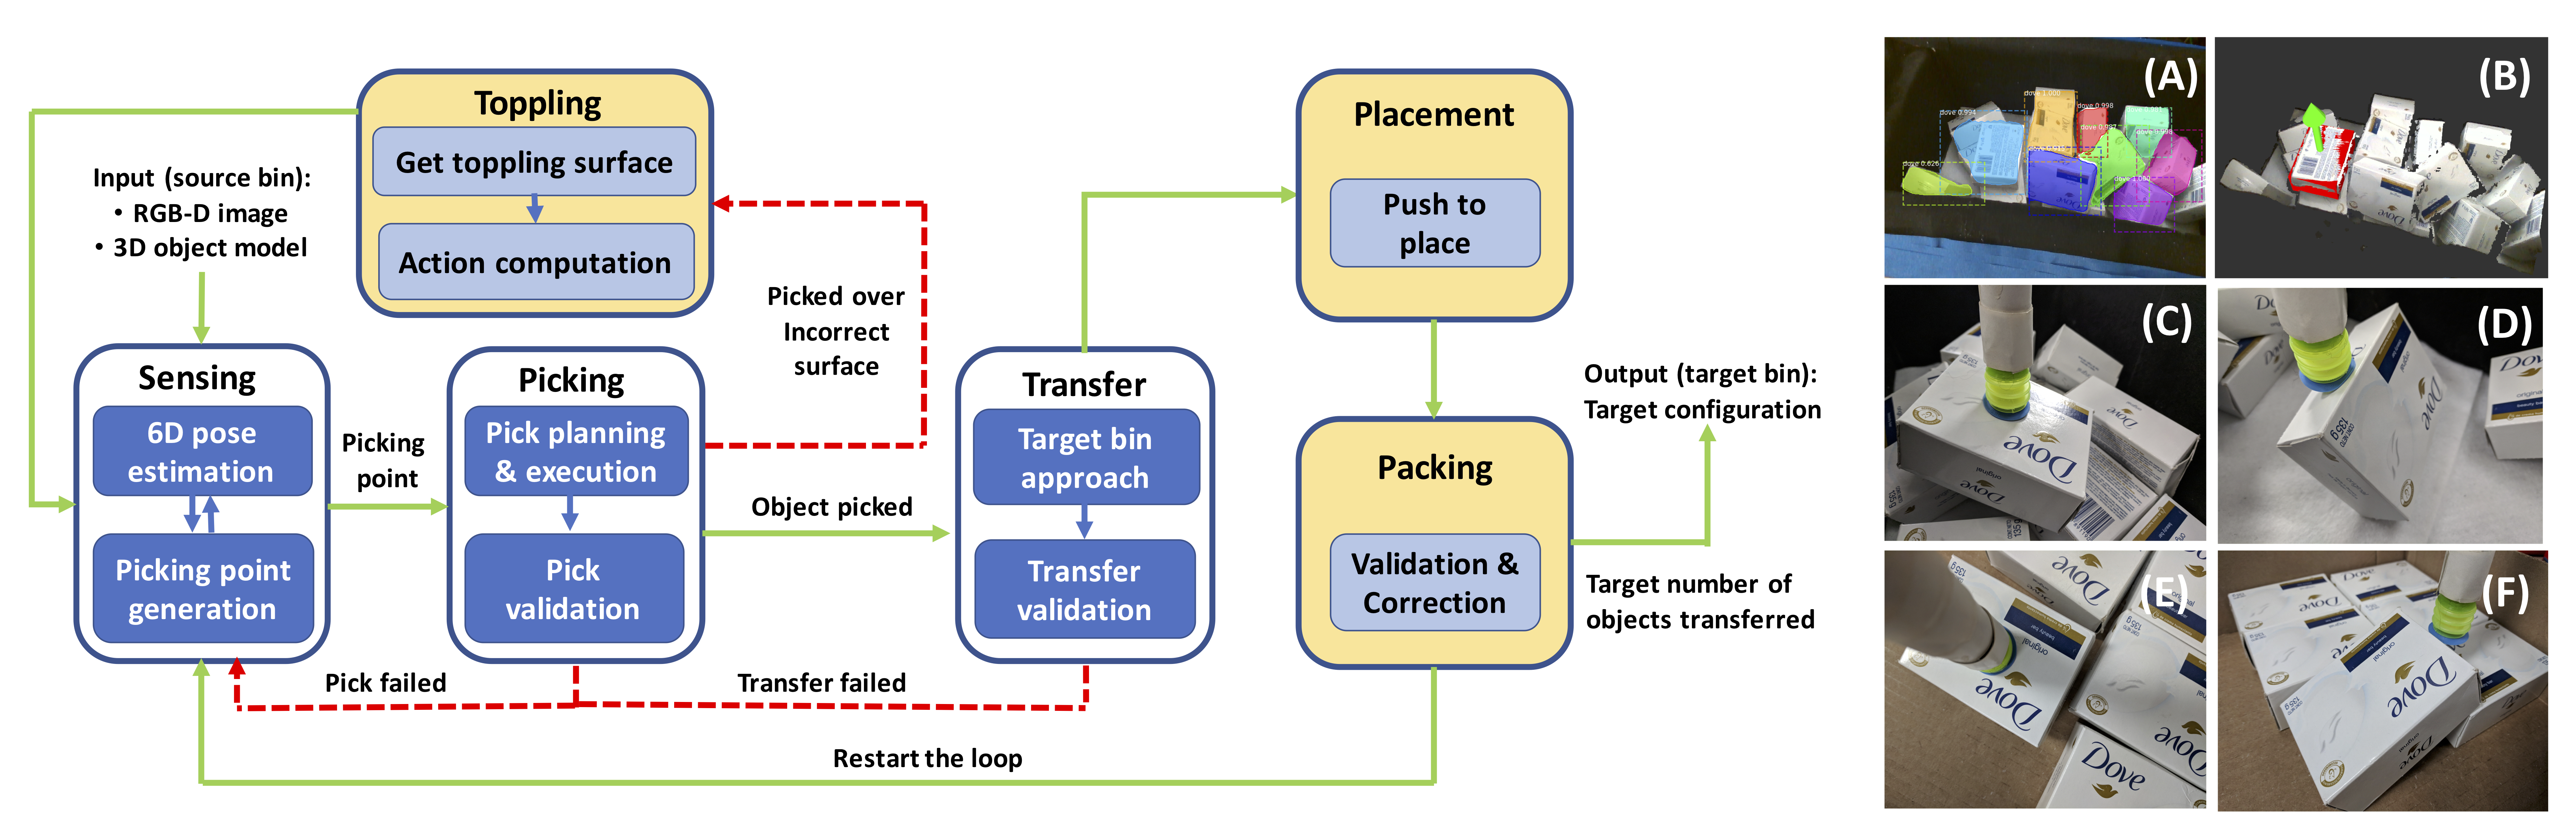
\includegraphics[width=1\textwidth]{Figures/final_pipeline.png}
\vspace{-0.1in}
\caption{\textit{Left}: Pipeline in terms of control, data flow (green lines) and failure handling (red lines). The blocks identify the modules of the system. Sensing receives an RGBD image of $\binit$ and object CAD models to return a grasp point. Based on the picking surface, the object is either transferred to $\btarget$ or is handled by the {\tt Toppling} module, which flips the object and places it back in $\binit$. When the object is transferred, a robust {\tt Placement} module places the object at the target pose $\hat{p}^i$. The Packing module validates and corrects the placement to achieve tight packing. \textit{Right}: a) Instance segmentation. b) Pose estimation and picking point selection are provided by sensing, c) Picking d) Toppling e) Placement and f) Packing.
}
\vspace{-0.2in}
\label{fig:pipeline}
\end{figure*}

Consider a robotic arm in a workspace $\Wspace$ with known static obstacles, two bins $\binit$ and $\btarget$, as well as $n$ movable, uniform objects $\objectset=\{ \object^1, \ldots, \object^n \}$ of known cubic dimensions. The bins $\binit$ and $\btarget$ are static but also compliant bodies in known poses that define a cuboid volume in $\Wspace$ where the objects can be placed. 

A labeled arrangement $\arrangement = \{ \pose^1, \ldots, \pose^n \}$ is an assignment of poses $\pose^i \in SE(3)$ to each object $\object^i$. Initially, the objects are in a start arrangement $\ainit$, where the objects are inside $\binit$ in random but ``stable'' poses, i.e., the objects are stably resting and not moving. The $\ainit$ arrangement is \emph{not} known a-priori to the robot. 

The objective is to move $\objectset$ to an unlabeled arrangement $\atarget = \{ \hat{\pose}^1, \ldots, \hat{\pose}^n \}$, which achieves a tight packing in $\btarget$. $\atarget$ depends on the pose of $\btarget$, its dimensions and the object dimensions. The target arrangement and the picking order is input for the proposed process. The target arrangement maximizes the number of objects inside  $\btarget$, while the objects rest on a stable face, and minimizes the convex hull of the volume the objects $\objectset$ occupy in $\Wspace$. This is typically a grid-like regular packing for cuboid objects. The unlabeled nature of $\atarget$ means it is satisfied as long as one of the objects is placed at each target pose, i.e.,

\vspace*{-5mm}
\begin{equation}
\forall \hat{\pose}^j \in \atarget: \exists\  \object^i \in \objectset \textrm{ so that } D(\hat{\pose}^j, p^i) < \epsilon,
\label{eq:satisfaction}
\end{equation}

\noindent where $\epsilon$ is a threshold for achieving the target poses; $D(\cdot,\cdot)$ is distance between object poses, which should consider the 3-axis symmetry of the cubic objects. In particular, if two poses result into an object occupying the same volume, then their distance is 0. For instance, rotation by $\pi$ about the vertical axis for a stably resting cube on a flat surface results in distance 0. A popular distance metric for 6D poses is the ADI metric ~\cite{hinterstoisser2012model}. The evaluation section will describe the distance used in the experimental process for evaluating the error of the final arrangement given point cloud data.

%, i.e., any rotation by $\pi$ about any axis perpendicular to an object surface that goes through its center results in the same volume being occupied. The experimental section will provide more details on the evaluation of this distance function given sensing data.   

%, where  $\cfull$ is the space of all possible arm configurations $q \in \cfull$

The arm has $d$ joints that define the arm's configuration space $\cfull \subset \mathbb{R}^d$, which has a collision-free subset $\cfree$. Valid arm motions correspond to a continuous C-space curve $\pi : [0,1] \rightarrow \cfree$.  The arm has an end-effector, such as a suction cup, for which discrete operations $\{ \mathtt{pick}, \mathtt{release} \}$ give rise to discrete modes: $\mathcal{M} = \{ \mathtt{transfer}, \mathtt{transit} \}$. No within hand manipulation operations are available. The state space of the arm is: $\mathcal{X} = \cfree \times \mathcal{M}$. Sensing is used to reason about the current object poses. Overall, the robot operations involve (i) moving the joints, (ii) picking or releasing objects and (iii) sensing.

%technology $S: \Wspace \rightarrow \mathcal{I}$, such as {\tt RGB-D} cameras, that can generate a representation  $\mathcal{I}$ of the workspace $\Wspace$, such as images, that allow 

The arm's forward kinematics define a mapping $\fk: \cfull \rightarrow SE(3)$, which provides the pose $g \in SE(3)$ of the end-effector given $q \in \cfull$. The reachable task space defines the end-effector poses the arm can reach without collisions: $\mathcal{T} = \{ \forall\ q \in \cfree: FK(q) \in SE(3)\}.$ For the arm to pick $\object^i$ at $\pose^i$, it has to be that the arm's end-effector pose $\grasp$ satisfies a binary output function: $\mathtt{is\_pick\_feasible}( \object^i, \pose^i, \grasp), \textrm{ where } \grasp \in \mathcal{T}.$ For instance, the pose $\grasp$ of a suction cup must align it with at least one of the surfaces of an object $\object^i$ at $\pose^i$. Then, it is possible to define the set of end-effector poses, which allow to pick an object at a specific pose: $$\graspset( \object^i, \pose^i ) = \{\grasp \in \mathcal{T}:  {\mathtt{is\_pick\_feasible}}(\object^i, \pose^i, \grasp) = true\}.$$ 

Assume the sets $\graspset( \object_i, \pose_i )$ are non-empty for all objects $\objectset$ and poses in $\ainit$ or $\atarget$ (and their vicinity inside bins $\binit$ and $\btarget$). Otherwise, the task is not feasible. Note that it may be necessary to reconfigure the objects inside the initial bin so as to pick them from the appropriate face before placing them. This is due to the lack of within-hand manipulation.

Given the above definitions, the task is to identify a sequence of motions for the arm as well as end-effector and sensing operations to transfer the objects  $\objectset$ from the unknown initial stable arrangement $\ainit$ inside $\binit$ to a tight, grid-based packing inside $\btarget$ defined by an unlabeled arrangement $\atarget$, so as to satisfy Eq. \ref{eq:satisfaction}.  

\section{System Components}
\label{section:Pipeline}
This section describes critical components that influence the design of the proposed pipeline:

\paragraph{Hardware Setup}
The robot used in the setup is the $\mathtt{Kuka\ IIWA14}$ $7$-DoF arm (Fig.~\ref{fig:new_setup} middle). A customized end-effector solution extrudes a cylindrical end-effector that ends with a compliant suction cup, to engage vacuum grasps. Two \textit{RealSense} \commentadd{SR300} cameras are mounted on a frame and pointed to containers $\binit$ and $\btarget$ from the other side relative to the robot as Fig.~\ref{fig:new_setup} (right) shows. While far from the robot, the cameras' frame is statically attached to the robot's base such that calibration errors are minimized in estimating the camera poses in the robot's coordinate system. 

% A high-power compressor and valve mechanism is used to generate powerful suction forces at the end-effector.

\paragraph{Workspace Design}
Fig.~\ref{fig:new_setup} (right) shows the setup designed for the target task. The annular blue region represents the subset of the reachable workspace that allowed for top-down picks with the robot's end-effector. This region is computed by extensively calling an inverse kinematics (IK) solver for top-down picks with the end-effector. The IK solutions indicate that the radial region between $40cm$ and $70cm$ from the robot center maximizes reachability and IK solution success given the setup.  The bins (red rectangles) are placed so that they lie inside the optimal reachable region. 

%This promotes picking strategies that approach the bins from the top.

% \subsection{Pose Estimation}
% The captured RGB-D data is passed through a convolutional neural network trained to perform object segmentation at the image level. This work has explored problems involving multiple object classes, and multiple instances of the same object, utilizing state-of-the-art solutions, such as {\tt FCN}~\cite{long2015fully} and {\tt MaskRCNN}~\cite{he2017mask}. Out of all the detected segments with a confidence threshold, only one is selected that is heuristically most promising for overhand picks. The heuristic criteria maximize the mean global Z-coordinate of all the RGBD pixels in the segment. Pose estimation~\cite{175}\cite{stocs} is performed over the selected segment (see Fig.~\ref{fig:pipeline}). The estimation returns a registered point set in the observed data, corresponding to the retrieved object model. 

% \subsection{Pick Selection}
% Using the corresponding set of mesh points, the one with the best pick score is chosen. Scoring calculates the distance to the center of the object mesh. A continuous neighborhood of planar pickable points is required to make proper contact between the suction cup and the object surface. A local search is performed around the best grasp score point, to then maximize the pickable neighborhood.

\paragraph{Software}
{\tt MoveIt!}~\cite{chitta2012moveit} is used for motion planning. Most of the motions are performed using \textit{Cartesian Control}, which guides the arm using end-effector waypoints. Ensuring the motions occur in reachable parts of the space increases the success of \textit{Cartesian Control}, simplifies motion planning and speeds-up execution. To decrease planning time, motion between the bins is precomputed using the $\mathtt{RRT^*}$ algorithm~\cite{Karaman2011Sampling-based-} and simply replayed at appropriate times. 

% At runtime, the framework computes only actions for moving the end-effector from a predefined pose above each bin either to a picking or a placing configuration. 

% \subsection{Task Planning}
% The pipeline described in Fig.~\ref{fig:pipeline} shows the sequence of task planning steps undertaken to perform continuous Pick-and-Place. The gray circles represent the control junctures between which motion and sensing is parallelized. Instead of waiting for the sensing and grasp generation, both are invoked asynchronously at the beginning of moving to the source bin. Once the motion ends, the grasping point is available for planning purposes. The pipeline keeps trying to detect new grasps till no further segments can be detected in the scene, which indicates that the source bin is empty.


\section{Proposed Solution}
\label{section:solution}
The proposed pipeline, described in Fig.~\ref{fig:pipeline}, provides the steps undertaken to perform the desired packing. The baseline steps correspond to: 
\begin{myitem}
\item[a)] {\em (Sensing)}: sense and select a target object $o^i$ to pick up;
\item[b)] {\em (Picking)}: execute action $\{\tt pick\}$; 
\item[c)] {\em (Transfer)}: move $o^i$ to the next available target pose $\hat{p}^j$ and execute action $\{\tt release\}$.
\end{myitem}
The experimental section considers this baseline pipeline, where it is observed that it performs poorly due to multiple sources of uncertainty, ranging from pose estimation and calibration errors, to object non-uniformity and object interaction with the bin and other objects, among others. These issue necessitate the introduction of remedies, which actively reduce the impact of the uncertainty. To this end, 3 manipulation primitives for a simplistic end-effector are designed to increase robustness and are integrated with the overall architecture: 
\begin{myitem}
\item[i)] Toppling;
\item[ii)] Robust Placement; and 
\item[iii)] Corrective Packing.
\end{myitem}

%\subsection{Baseline - Without Pose Estimation}
%A placement module informs the task planner of the position and orientation of the dropped objects.After an object is picked up, the robot will directly move to the target position and drop the object. 

%\subsection{Packing While Trusting Pose Estimation}
%For different objects, the transform between the grasped object and the end-effector is different, given the target pose of the object, adjustments of the pose of the grasped object can be done to attempt to align it to the desired drop positions.

\subsection{Baseline: Pose Estimation and Picking}
Given an RGB-D image of the source bin and a CAD model of the object, the objective is to retrieve ($\object^i$, $\pose^i$) such that it maximizes the chance of achieving target configuration $\hat{p}^j$, where $D(p^i,\hat{p}^j) \leq \epsilon$. To achieve this, the image is passed through a {\tt MaskRCNN} convolutional neural network~\cite{he2017mask}, which is trained to perform segmentation and retrieve the set of object instances $\objectset$.  An image segment is ignored if it has a number of pixels below a threshold. It is also ignored, if {\tt MaskRCNN} has small confidence that the segment corresponds to the target object. Among the remaining segments, instances $\object^i \in \objectset$ are arranged in a descending order of the mean global Z-coordinate of all the RGBD pixels in the corresponding segment. Then, 6D pose estimation is performed for the selected instance~\cite{175}\cite{stocs}. 

If, given the detected 6D pose of the instance, the top-facing surface does not allow the placement of the object via a top-down pick, the next segment instance is evaluated in order of the mean global Z-coordinate. If no object reveals a top-facing surface, then the first object in terms of the maximum mean global Z-coordinate is chosen for picking. 

For the selected object, a picking point, i.e., a point where the suction cup will be attached to the object, is computed over the set of points registered against the object model. It utilizes a picking-score associated in a pre-processing step with each model point, which indicates the stability of the pick on the object's surface. The score calculates the distance to the center of the object mesh. A continuous neighborhood of planar pickable points is required to make proper contact between the suction cup and the object surface. Thus, a local search is performed around the best pick-score point to maximize the pickable surface.


% For the arm to pick $\object^i$ at $\pose^i$, it has to be that the arm's end-effector pose satisfies certain conditions relative to the object's pose as expressed by a binary output function: $\mathtt{is\_pick\_feasible}( \object^i, \pose^i, \grasp), \textrm{ where } \grasp \in \mathcal{T}.$ For instance, the pose $\grasp$ of a suction cup must align it with at least one of the surfaces of an object $\object^i$ at $\pose^i$. Then, it is possible to define the set of end-effector poses, which allow to pick an object at a specific pose: \vspace{-.05in}$$\graspset( \object^i, \pose^i ) = \{\grasp \in \mathcal{T}:  {\mathtt{is\_pick\_feasible}}(\object^i, \pose^i, \grasp) = true\}. \vspace{-.05in}$$ 

% Assume the sets $\graspset( \object_i, \pose_i )$

\subsection{Toppling}
% \commentadd{
% An error in the picking action or the absence of objects exposing top-facing surfaces allowing placement of the object with a single pick, necessitates a strategy to expose a desired pickable surface of the object.
% }
\rahul{
% \begin{figure}
%     \centering
%     \includegraphics[width=0.3\textwidth]{Figures/toppling_begin.png}
%     \includegraphics[width=0.3\textwidth]{Figures/toppling_end.png}
%     \caption{An illustration of a scene where a direct pick-and-place fails to solve the problem without reorienting the object. The \textit{top} image shows the initial scene where the orange cuboidal object needs to be transferred to the target bin at the pose denoted by the wireframe marker. The \textit{bottom} image shows the end-effector placing it using a top-down grasp.}
%     \label{fig:reorientation_failure}
% \end{figure}
}
The toppling primitive is invoked if there exists no object that exposes the desirable top-facing surface, or if the object was erroneously picked from the wrong face. The latter is detected after the pick by performing pose estimation once the objet is attached to the suction cup. For instance this can happen for the soaps shown in Figure \ref{fig:pipeline} (right)(d), if the thin side is available for pick but the soap needs to be placed on their wider side. In this case, a toppling primitive is used to reorient the object.
\rahul{
% \begin{figure*}
%     \centering
%     \includegraphics[width=0.24\textwidth]{Figures/toppling1.png}
%     \includegraphics[width=0.24\textwidth]{Figures/toppling2.png}
%     \includegraphics[width=0.24\textwidth]{Figures/toppling3.png}
%     \includegraphics[width=0.24\textwidth]{Figures/toppling4.png}
%     \caption{Steps of toppling primitive from left to right. \textit{Firstly,} the scenario where the grasped pose of the object does not allow the target placement is detected, \textit{secondly,} a plane is detected in the scene that can allow toppling, \textit{thirdly,} the toppling direction is computed and executed, and \textit{finally,} the reoriented object rests in a pose that allows the target placement.}
%     \label{fig:toppling_steps}
% \end{figure*}

\begin{figure*}
    \centering
    \includegraphics[width=1\textwidth]{Figures/toppling}
    \caption{Steps of toppling primitive from left to right when the scenario where the grasped pose of the object does not allow the target placement is detected. \textit{Firstly,} a plane is detected in the scene that can allow toppling, \textit{secondly,} the toppling direction is computed and \textit{thirdly} executed, and \textit{finally,} the reoriented object rests in a pose that allows the target placement.
    An illustration showing the toppling vector computation with (a) shows the dimensions of the object with \textit{s} being the dimensions along the side that exposes a desired face, and \textit{z} being the height of the top face. On the right, (b) shows the topping vector under the assumption that the object was grasped from the center of the face.
    }
    \label{fig:toppling_steps}
\end{figure*}
}

% The candidate object $o^i$ should be transferred if its detected pose $\pose_{start}$ allows, when moved to $\btarget$, to the next available target pose $\hat{p}^j$. But it could be that while $\graspset( \object^i, \pose_{start} ) \neq \emptyset$, the pose $\pose_{start}$ does not allow the arm to move the object to the target bin in a way that to achieve $\hat{p}^j$. 
% }
% For instance this can happen for the soaps shown in Figure \ref{fig:pipeline} (right), if the thin side is available for pick but the soap needs to be placed on their wider side. 
% In this case, a toppling primitive is used to reorient the object. The toppling primitive is invoked if there exists no object that exposes the desirable picking surface, or if the object was erroneously picked from the wrong face, which is detected after the pick by performing pose estimation on it. 
%Taking into account reachability, collisions and limited symmetry relaxations $\mathbb{P}_{INV}$ can be significantly large enough. A packing method cannot be complete unless there is some explicit reasoning about this set of poses.
%Within the classes of available actions $\{ \mathtt{pick}, \mathtt{release} \}$ a fixed attachment is enforced during a $\mathtt{pick}$, and the constraint is removed during a $\mathtt{release}$. 
% \commentadd{
% Given a starting pose of an object $\pose_{start}$, let the operation $\pose_{topple} = \mathbb{TR}(\pose_{start}, \Pi_{start} )$ represent the pose of the object at the end of the set of actions $\Pi_{topple}: [0,1] \rightarrow \mathcal{X}$ of the arm, defined in the full state space. A toppling action sequence $\Pi_{topple}$ attempts to find a sequence of motions that bring the pose of the object $o^i$ to $\pose_{topple} = \mathbb{TR}(\pose^i, \Pi_{topple} )$, so that:
% % \vspace*{-5mm}
% \begin{equation}
% \exists\ \Pi_{transfer}, \textrm{ so that } D( \mathbb{TR}( \pose_{topple}, \Pi_{transfer} ), \hat{p}^j)  \leq \epsilon
% \label{eq:topple}
% \end{equation}
% }

Given a starting pose of an object $\pose_{start}$ and a toppling action of the arm, the object ends up at a new pose $\pose_{topple}$. The objective is to allow the existence of a pick $\hat{g} \in \graspset( \object^i, \pose_{topple} ) $ so that there is a $\mathtt{transfer}$ action from pick $\hat{g}$ that achieves the final  placement $p_{end}$ close enough to the desired target placement $\hat{p}^j$, i.e., $D(p_{end},\hat{p}^j) \leq \epsilon$. For the considered setup, this means that the top-facing surface of the object at $\pose_{topple}$ and $\hat{p}^j$ is the same.

The toppling module inspects the visible point cloud in the source bin to identify the best toppling plane, which is sufficiently empty and flat. The accompanying implementation restricts actions to ones that change the pose of the cubic objects by shifting the most upward facing surface to only one of the adjacent surfaces. While this does not guarantee toppling the object to all possible poses, the symmetry of cubic products resolves this issue. 

Prior work \cite{lynch1999toppling} has shown the efficacy of minimal end-effectors used in tandem with the environment to achieve toppling. In the previous work, the friction against a conveyor belt is used to topple an object about a resting surface. The conveyor belt's motion is parallel to the initial resting surface plane. In the current setup, the compliance of the suction cup is used to emulate the same effect using a lateral motion on the same plane as the top-surface along the direction of the desired transformation between $\pose_{start}$ and $\pose_{topple}$. Due to symmetry, at least one neighboring surface allows top-down picks, so a successful toppling action exists. Using the pose of the object, the lateral motion direction is executed once the object is placed on the detected plane, and the object is released during this action. Results show that this is highly effective in the target setup.

% of satisfying Eq. \ref{eq:topple}. 

% A high level subroutine in the context of the pipeline is demonstrated as follows.



\rahul{
% \begin{figure}[t]
%     \centering
%     \includegraphics[width=0.48\textwidth]{Figures/toppling_direction.png}
%     \caption{An illustration showing the toppling vector computation with (a) shows the dimensions of the object with \textit{s} being the dimensions along the side that exposes a desired face, and \textit{z} being the height of the top face. On the right, (b) shows the topping vector under the assumption that the object was grasped from the center of the face.}
%     \label{fig:toppling_direction}
% \end{figure}

Algorithm~\ref{algo:topple} describes the high-level sequence of steps involved in executing a toppling action. This subroutine will be invoked once the object is already attached to the end-effector using a top-down grasp, and is also visible to the camera in order to obtain a point cloud. It returns a sequences of poses that constitute the discrete steps of the toppling maneuver, which when executed should drop the object to expose a desired face, denoted by the target orientation.
Line 2 checks whether such a reorientation is even necessary by using the symmetry aware distance between the current grasped pose, and the desired pose. The toppling plane is obtained by estimating a large enough (based on the dimensions of the bottom surface of the object) planar surface on the point cloud, that is also priorized to prefer lower planes than expectedly more unstable higher surfaces on the pile. 

The {\tt GetOffset} primitive is described in Fig~\ref{fig:toppling_steps} (second) to show the computation of the toppling maneuver. Given the pose of the object, the height of the top face is denoted by \textit{z}. Given the desired face(s) that needs to be exposed as the top face to allow the target placement using a top-down grasp, \textit{s} denotes the dimension of the edge(s) not adjacent to the desired face; i.e., out of the two dimensions defining the top-face, select the one that corresponds to the direction of toppling. Define $\theta = \tan^{-1} \frac{s}{z} $. The toppling has to change the orientation of the object till its center (approximating the center of gravity) goes beyond the support point at along the contact edge denoted by the white circle in the image. This object rotation can be affected by displacing the grasp point of contact (green circle) to the {toppled configuration} (red circle). Without loss of generality, consider the point of grasp to be the center of the top face. The offsets become:

\vspace{-0.2in}
$$
	\Delta x = \frac{s}{2} + z \sin \theta - \frac{s}{2} \cos \theta + \epsilon;\ 
	\Delta z = z \cos \theta + \frac{s}{2} \sin \theta - z
$$
\vspace{-0.15in}

Here $\Delta x$ and $\Delta z$ denote the planar and height offsets in the object's local frame describing the toppling vector, shown by the red arrow in Fig~\ref{fig:toppling_steps} (third). $\epsilon$ is meant to allow some error tolerance to the maneuver, when the action is executed by pivoting the object. 

 \begin{algorithm}
 \small
 \DontPrintSemicolon
 \KwIn{Point cloud $C$, object $\object$, top-down current object pose $\pose\gets(t,r)$, target orientation $r_{\mathrm target}$}
 \KwOut{Toppling primitive $\Pi$  }
 	$\Pi\gets\emptyset$;\\
 	\If{ $D$($\pose, (t,r_{\mathrm target}$)) $\ >\ \epsilon $ }
 	{
 		$t_{\mathrm plane} \gets ${\tt GetTopplingPlane}($C, ${\tt Dimensions}($\object$));\\
 		$\pose_{\mathrm plane} \gets (t_{\mathrm plane}, r)$\\
 		$\Pi \gets \Pi \cup \pose_{\mathrm plane}$;\\
 		$(\theta,\Delta x,\Delta z) \gets ${\tt GetOffset}($\object, \pose_{\mathrm plane}, r_{\mathrm target}$);\\
 		$\Pi \gets \Pi \cup $ {\tt ApplyOffset}($\pose_{\mathrm plane}, \theta,\Delta x,\Delta z$);
 	}
 \Return{$\Pi$}
 \caption{{\sc Topple}}
 \label{algo:topple}
 \end{algorithm}

}

% Put ee in image


% There may exist a set of objects in $\objectset$ that require regrasping, because the initial pose of the object $\pose$ in $\ainit$ does not allow any valid grasp that allows a prehensile transfer to the target pose. In such situations, the current solution detects instances where the objects of the source bin are not desirably graspable, raises them above the source bin, tilts and drops them. This maneuver attempts to change the pose of the object to an orthogonal one, which by the nature of symmetry of cuboidal objects, should expose a desirable face to top-down grasps. Once an object's pose is successfully changed to one that allows a transfer to the target bin, the lower levels of the task planning hierarchy can deal with it. 

% Consider an object $\object$ at pose $\pose_{init}$, and $\pose_{goal}$ be the target pose in the context of packing the object in $\btarget$. If it is detected that $\graspset_\object^{\pose_{init}} \cap \graspset_\object^{\pose_{goal}} = \emptyset$, there can be no grasp that can transfer the object. The regrasp task is defined as the sequence of transfers and moves that the object from the initial pose, $\pose_{init} \in \ainit$ to some intermediate pose $\pose_{k}$ at the end of a valid motion of the arm, $\pi_{regrasp}$ such that
% $$
% \pose_k \in \amove_{\pi_{regrasp}}^{\ainit}, \graspset_\object^{\pose_{k}} \cap \graspset_\object^{\pose_{goal}} \neq \emptyset
% $$
% Once the object is at $\pose_k$ a transfer $\pi_T$ can place it in $\pose_{goal}$.
% This operation is applied to all objects in $\objectset$ that require regrasps in order to ensure every object is successfully packed into the target bin. 


\subsection{Point Cloud Driven Adaptive Pushing}
\begin{figure*}[t]
\centering
\begin{overpic}[height=1.2in]{Figures/step_1}%
\put(350,-100){(a)}%
\end{overpic}
% \includegraphics[height=1.2in]{Figures/step_1}
\begin{overpic}[height=1.2in]{Figures/push_3.png}%
\put(350,-100){(b)}%
\end{overpic}
\hspace{0.1in}
% \includegraphics[height=1.2in]{Figures/push_3.png}
\begin{overpic}[height=1.2in]{Figures/tight_push_00.png}%
\put(450,-70){(c)}%
\end{overpic}
% \includegraphics[height=1.2in]{Figures/tight_push_00.png}
\begin{overpic}[height=1.2in]{Figures/tight_push_02.png}%
\put(450,-70){(d)}%
\end{overpic}
% \includegraphics[height=1.2in]{Figures/tight_push_02.png}
\begin{overpic}[height=1.2in]{Figures/tight_push_03.png}%
\put(450,-70){(e)}%
\end{overpic}
% \includegraphics[height=1.2in]{Figures/tight_push_03.png}
% \vspace{-0.1in}
\caption{Adaptive pushing: (a) The black border is the bin and the gray rectangle a previously placed object. The green rectangle represents the target pose for the current object. The light green boundary represents an $\varepsilon$-expanded model that intersects the point cloud at the purple points. These points result in the black vector that pushes the object away from them. (b) A screen shot of a scene's point cloud, where the white points are collision points with previously placed objects and the red volume shows the computed pre-push pose for the new object.
Adaptive pushing in the boundary case (the sixth object). (c)The target object is moving at the upper level and from the pre-push pose to the boundary. (d) The target object is being pushed against the boundary and then pushed down to the bottom level. (e) The target object is moved towards its target pose at the bottom level.
}
\label{fig:adaptive-pushing}
% \vspace{-0.2in}
\end{figure*}



%In the problem of packing in a tight space, failures tend to arise due to the uncertainties from perception of the object and the environment. In order to increase the robustness of packing, we propose a novel manipulation primitive we call "Push-Place". This primitive takes advantage of the compliance of the objects and environments to robustly placing an object in a tight bin. The idea is that instead of directly placing the object to its target position, while still attaching the object to the end-effector, we will first move the object to an intermediate position, then push the object towards its target position. This method has two main benefits: first, in finding the intermediate position, we minimize the probability of collision between the object and the environment;second, during the course of pushing, in addition to moving the target object to its desired position, the interaction between objects will also correct the misalignment of previous packed objects.     

Directly placing objects at the goal pose $\hat{p}^i$ into bin $\btarget$ is prone to placement failures due to errors in perception as well as prior placements. This may result in damaging the objects. A safer alternative is to drop the object from a certain height, right above the goal pose, so as to avoid pressing against previously erroneously placed objects. Still, however, this alternative results in low quality packing. A key realization is that during placement, the object being manipulated will inevitably approach or even collide with other objects or the target container. To sidestep undesirable collisions, an {\em adaptive pushing} primitive is developed, which directly operates over point cloud data for the target bin. 


The process is detailed in algorithm~\ref{algo:PushPlace}. The adaptive pushing begins by growing the object model at the target pose $\hat{p}^i$. Given the uncertainty value $\varepsilon$, the model is enlarged by  $2\varepsilon$ along each dimension. The enlarged model is intersected with the point cloud to retrieve collision points. A collision vector is computed as a vector pointing from a collision point to the center of the object model. Summing all collision vectors yields the displacement vector. By iteratively moving the object model along the unit displacement vector, where the displacement vector is recomputed after each movement, a collision-free pre-push pose for the object is obtained. An example scene is shown in Fig.~\ref{fig:adaptive-pushing}. During the execution, the robot first moves the object above the pre-push pose, then lowers the object to the pre-push pose and finally pushes the object to the target pose. 

% The adaptive pushing primitive begins by moving the picked-up object to a pose with a larger $z$-value than the goal pose $\hat{p}^i$. It then tries to find a set of intermediate target poses for generating collision-free paths for the object and the end-effector as the object is gradually lowered to its final desired pose. The idea behind generating one such intermediate pose is shown in Fig.~\ref{fig:adaptive-pushing}, where a {\em displacement vector} is shown. At any point when a new intermediate pose is to be generated, to counter the potential negative effects caused by pose uncertainty, an $\varepsilon$-expanded model of the object's current estimated pose (i.e., growing the object model by $2\varepsilon$ along each dimension) is intersected with the point cloud. Based on the intersection, a displacement vector defining a new intermediate pose is  generated that guides the object away from potential collisions. 

%An intermediate pose is denoted a {\em pre-push pose}. Algorithm~\ref{algo:PushPlace} outlines the process of finding these pre-push poses. 

\begin{algorithm}
\small
\DontPrintSemicolon
\KwIn{Pointcloud $C$,  target pose $\pose_t$, bounding box size $S$}
\KwOut{Push direction $d$, pre-push pose $\pose_{pre}$  }
$\pose_{pre} \gets \pose_t$ \;
 $bbox \gets$ GenerateBoundingBox($\pose_{pre}, S$)  \;
\While{$bbox$ \normalfont is in collision}{
$C_{collision} \gets$ Intersection($bbox , C$) \;
 $u_{push} \gets$ GeneratePushVector($C_{collision}, \pose_{pre}$)\;
 $\pose_{pre} \gets \pose_{pre} + u_{push}$\;
 \lIf{\normalfont IsLocalMinimum($\pose_{pre}$)}{
    decrease $S$
 }
 $bbox \gets$ GenerateBoundingBox($\pose_{pre}, S$)
}
$d \gets \pose_t - \pose_{pre}$\;
\Return{$d, \pose_{pre}$}\;
\caption{{\sc PushPlace-Planner}}
\label{algo:PushPlace}
\end{algorithm}

\begin{algorithm}
\small
\DontPrintSemicolon
\KwIn{Pointcloud $C$,  target pose $\pose_t$, bounding box size $S$}
\KwOut{Push path $path$ }
$\pose_{higher} \gets \pose_{t}   $\;
$\pose_{higher}.z \gets \pose_{t}.z + obj\_height   $\;
$(d, \pose_{pre}) \gets$ PushPlace-Planner$($C$, \pose_{higher}, S)$  \;
$\pose_{wall} \gets$ ProjectPoseToWall($\pose_{higher})$   \;
$\pose_{down} \gets \pose_{wall}$  \;
$\pose_{down}.z \gets \pose_{wall}.z - obj\_height$   \;
$path \gets (\pose_{wall}, \pose_{pre})$   \;
$path \gets (\pose_{down}, \pose_{wall})$\;
$path   \gets (\pose_{t}, \pose_{down})$    \;
\Return{$path$}\; 
\caption{{\sc TightPushPlace-Planner}}
\label{algo:TightPushPlace}
\end{algorithm}


For special scenario where objects need to be packed tightly with no clearance, in order to place the objects near the boundary robustly, it requires additional steps in pushing. The process is detailed in algorithm~\ref{algo:TightPushPlace}. In this case, since there is no space for pushing in the same layer of the target pose, the target object will first be moved at the upper layer and use the boundary of the container to correct potential noise in the object pose. The compliance of the container boundary will also enable the object to fit the tight gap when the object is pushed down to target level. The process of placing one object to an boundary pose is illustrated in Fig.~\ref{fig:adaptive-pushing}. This procedure is required for each object that is at the boundary of the container. 

% \begin{figure}[t]
% \centering
% \includegraphics[width=0.15\textwidth]{Figures/tight_push_00.png}
% \includegraphics[width=0.15\textwidth]{Figures/tight_push_02.png}
% \includegraphics[width=0.15\textwidth]{Figures/tight_push_03.png}
% \vspace{-0.1in}
% \caption{Adaptive pushing in the boundary case (the sixth object). (left)The target object is moving at the upper level and from the pre-push pose to the boundary. (middle) The target object is being pushed against the boundary and then pushed down to the bottom level. (right) The target object is moved towards its target pose at the bottom level.}

% % A screen shot where the green volume is the ground truth pose for the object and the red one is where the object should be moved next.}
% %\label{fig:workspace}
% \label{fig:tight-pushing}
% \vspace{0.1in}
% \end{figure}

%Line 1-2 initialize the pre-push pose $\pose_{pre}$ and the bounding box $bbox$ generated at $\pose_{pre}$. The function GenerateBoundingBox generates a bounding box centered at the given pose with the given size. In line 2, the size $S$ is bigger than the actual size of the object to reflect the uncertainties of the estimated pose. Line 3-8 of the algorithm iteratively tries to find a collision-free pre-push pose. The strategy is to move the bounding box towards the direction that will decrease the collision region. In line 4, Function Intersection($bbox, C$) will calculate the intersection points between bounding box $bbox$ and the environment pointcloud $C$. $C_{collision}$ will be passed to function GeneratePushVector to generate a local unit vector to move the current pre-push pose. In function GeneratePushVector($C_{collision}, \pose_{pre}$), all the vectors from points of $C_{collision}$ to the pre-push pose $\pose_{pre}$ are normalized, the summation of all these unit vectors is returned as the local push vector $u_{push}$. Then $u_{push}$ is used to update the pre-push pose $\pose_{pre}$. At narrow region, this local optimization process can be stuck at local minimum. The strategy we used is to reduce the size $S$ for generating bounding box. In the experiments, this usually helped to find a valid pre-push pose.



%\subsection{Packing With Use Of Non-Prehensile Push}
\subsection{Fine Correction using Push and Pull Primitives}
%As a local optimization strategy, the dynamic pushing primitive does not provide %guaranteed success. In the semi-structured setup of this work, however, it %provides a significant boost to robustness. 

\begin{figure*}
\centering
\begin{tabular}{@{}c@{}c@{}}
%\cline{2-2}
& No corrective actions\\
\multirow{3}{*}{\includegraphics[width=0.24\textwidth]{Figures/finer_fix.pdf}}
& \includegraphics[width=0.75\textwidth,valign=t]{./Figures/res_step_adaptive.png}
\\\cline{2-2}
& Full pipeline\\
& \includegraphics[width=0.75\textwidth]{./Figures/res_step_full.png}
\\%\cline{2-2}
\end{tabular}
\caption{Fine layout adjustment and correction.}
\label{fig:finer_fix}
\end{figure*}

The final primitive deals with the remaining failure cases. Fine corrections are required because objects can be placed in incorrect poses due to unexpected collisions as well as calibration and pose estimation errors.  The proposed corrective manipulation procedure continuously monitors the scene and triggers corrective actions whenever necessary. 

%Even small alignment errors can have a domino effect on the  packing task and make the placement of remaining objects infeasible. 

\begin{comment}
\begin{wrapfigure}{r}{1.5in}
\vspace{-.2in}
\includegraphics[width=1.49in]{Figures/finer_fix.pdf}
\vspace{-.3in}
\caption{Fine layout adjustment and correction.}
\label{fig:finer_fix}
\vspace{-.15in}
\end{wrapfigure}
\end{comment}

The process first removes the background, the box, the robot's arm and end-effector from the observed point cloud and computes its surface normals.
The observed point cloud is then compared against the desired alignment of the objects in their target poses. As shown in Fig.~\ref{fig:finer_fix}, two types of misalignment errors can occur. The first type occurs when the top surface normal of an object is not perpendicular to the support surface. This error is corrected by pushing the object along a direction and for a distance computed based on its surface normal in a manner that makes it aligned with the support surface. 
The second type of error happens when a peripheral object is not entirely within the desired footprint of the pile. The proposed procedure systematically detects pivot points that are outside the desired footprint of the pile and pulls their objects inside accordingly. The correction is repeated until the point cloud is  aligned with the desired goal poses given a threshold
%$\epsilon$
\changkyu{$\tau$}, or a timeout occurs.

\changkyu{
% [changkyu] uncommented 

Given the alignment pose $\hat{\pose}^i$ which defines the six \textit{facets} $\hat{F}^i = \{\hat{f}_1^i,\dots,\hat{f}_6^i\}$ of the cubic, the pre-processed observation $\mathcal{I}$ is split into disjoint sets $\{X^i\}_{i=0}^n$ where $X^i$ is the point cloud cropped by $\hat{F}^i$ and $X^0$ is the remaining.
Starting with the furthermost point cloud $X^i$ from a pivot point $x_{pivot}$, e.g. the upper right corner of the box, we determine if it agrees with $\atarget$ by measuring the distance between the point cloud $X^i$ and the closest facet $\hat{f}_j^{i'}$ that is not in parallel to the xy-plane as well as the normal difference.
Once a disagreement is detected, an appropriate pushing or pulling action is executed as described in Algorithm \ref{algo:FinerFix}.
For example, the objects leaning against other objects, which accompany a significant normal disagreement, will be pushed away to be slipped, and the objects translated from its desired position will be pulled towards it.
The correction is repeated until all the observation agree with $\atarget$ or timeout.

{\small
\begin{algorithm}
\KwIn{
	$\atarget = \{ \hat{p}^1, \ldots, \hat{p}^n \}$, an error threshold $\tau$, the point cloud segments $\{X[i]\}_{i=0}^{n}$, a corner point $x_{pivot}$
}
\Repeat{Timeout}
{
Sort centers of $X[i]$ based on increasing distance to $x_{pivot}$;\\

	\For{$i\leftarrow 0; i\leq n; i\leftarrow i+1$}
	{
		{\scriptsize\tcp{Check if X[i] is not horizontally placed}}
		\If{ $\{x | normal(x).z < 1 - \epsilon, x \in X[i]\} \neq \emptyset$ }
		{
        Push segment $X[i]$ from a side to translate its center $x_c$  with  $\alpha \times normal(x_c)$, after projecting vector $normal(x_c)$ to the XY plane, and where $\alpha$ is a small constant; \\
			break
		}
		{\scriptsize\tcp{Check if X[i] is horizontally off-set}}
        Let object\_box($\hat{p}^{i'}$) be the closest target to $X[i]$, and let $\beta$ be the {\it Frechet distance} between $X[i]$ and object\_box($\hat{p}^{i'}$).\\
%		\If{ $X[i]$ does not fit with $\hat{p}^i$ }
		{			
			\If{$\beta > \tau$}
			{
				Pull $X[i]$ toward $\hat{p}^{i'}$ with distance $\beta$;\\
				break
			}
		}
	}
	break
}
\caption{Realignment}
\label{algo:FinerFix}
\end{algorithm}
}

}

\begin{comment}
{\small
\begin{algorithm}
\KwIn{
	$\atarget = \{ \hat{p}^1, \ldots, \hat{p}^n \}$, an error threshold $\tau$
}
\Repeat{Timeout}
{
Get {\tt RGB-D} input $\mathcal{I}$;\\
\For{$i := 1; i \leq n; i\leftarrow i+1$}
{
	{\scriptsize\tcc{X[i]: point cloud segment for $o^i$}}
    $X[i] \leftarrow \mathcal{I} \cap \text{object\_box}(\hat{p}^i)$,
	$\mathcal{I} \leftarrow \mathcal{I} \backslash X[i]$
    
}
$X[0] = \mathcal{I}$;\\
$x_{pivot}$ is any corner point in the convex hull of $\mathcal{I}$;\\
Sort centers of $X[i]$ based on increasing distance to $x_{pivot}$;\\

	\For{$i\leftarrow 0; i\leq n; i\leftarrow i+1$}
	{
		{\scriptsize\tcc{Check if X[i] is not horizontally placed}}
		\If{ $\{x | normal(x).z < 1 - \epsilon, x \in X[i]\} \neq \emptyset$ }
		{
        Push segment $X[i]$ from a side to translate its center $x_c$  with  $\alpha \times normal(x_c)$, after projecting vector $normal(x_c)$ to the XY plane, and where $\alpha$ is a small constant; \\
			break
		}
		{\scriptsize\tcc{Check if X[i] is horizontally off-set}}
        Let object\_box($\hat{p}^{i'}$) be the closest target to $X[i]$, and let $\beta$ be the {\it Frechet distance} between $X[i]$ and object\_box($\hat{p}^{i'}$).\\
%		\If{ $X[i]$ does not fit with $\hat{p}^i$ }
		{			
			\If{$\beta > \tau$}
			{
				Pull $X[i]$ toward $\hat{p}^{i'}$ with distance $\beta$;\\
				break
			}
		}
	}
	break
}
\caption{Realignment}
\label{algo:FinerFix}
\end{algorithm}
}
\end{comment}

\section{Simulation Framework}
\label{section:simulation}
\rahul{A simulation framework is developed that models the physical aspects of real-world tight packing. Given the focus of developing and evaluating sensor-based control algorithms such as {\it adaptive pushing} and {\it fine-correction}, the framework simulates an RGB-D sensor to capture the state of packing. Fig.\ref{fig:simulator} shows the simulation setup in Blender \footnote{\url{http://www.Blender.org}}. 

The software framework loads a model of the {\it Bin} into the simulation environment. A {\it point lighting source} and a {\it camera} are initialized based on the parameters specified in a configuration file. A target packing sequence is specified for objects with known 3d models as $\{ (o_i, P_i) | i=1:K\}$, where $o_i$ identifies the object and $P_i$ denotes the desired target pose of the object. An example of the desired configuration is shown in Fig.\ref{fig:simulator} (left). 

An intermediate simulation state corresponds to the partial placement of objects in the bin. The achieved placement might be inaccurate due to the noise (artificially added in the simulation framework) from execution or sensing. The resulting state is captured via an RGB-D rendering of the scene. The simulation can either be set to render images via a fast rasterization-based rendering process or to generate photorealistic images via a physically based rendering. Additionally, the simulator generates depth images, instance segmentation masks and consequently the 3d point cloud data. This state information is provided as an input to a {\it control algorithm} such as adaptive pushing or fine correction. The control algorithm generates a motion of the end-effector for the placement of the target object which is then physically simulated via the Bullet Physics Engine \footnote{\url{http://www.bulletphysics.org}}. 

The simulator reasons about the physical interactions between the end-effector and the object being manipulated as well as the interactions between different objects. The simulator is developed to mimic the compliance of the real-world setup as shown in Fig.\ref{fig:simulator} (right). This is achieved by introducing a {\it spring constraint} between the end-effector and the object being manipulated. The spring constraint allows the link between the end-effector and the object to be stretched during the packing operation which is similar to the behavior achieved by the soft suction gripper. In the absence of this constraint, i.e. in a strictly rigid simulation, the objects would pop out to resolve the collision.}
\begin{figure*}[h]
\centering
\includegraphics[width=\textwidth]{Figures/simulator.pdf}
\caption{Simulator environment is setup with a bin, lights and camera parameters. Objects are placed sequentially to achieve a desired target configuration. Before each placement, the state of the bin is captured by rendering RGB-D images. The state is provided as input to the control algorithm that computes the motion for the target object. Finally, the controls are executed in the simulator to place the object in the bin. To accurately model the compliance of the real-world end-effector, a spring constraint is applied in simulation between the end-effector and the object. The constraint allows small relative motion and prevents unrealistic collision and jumping of objects that are often observed in rigid-body simulation.}
\label{fig:simulator}
\end{figure*}



\section{Evaluation}
\label{section:evaluation}
To evaluate the performance of the proposed pipeline, extensive experiments were executed on the \kuka platform of Fig. \ref{fig:new_setup}, to accurately represent the motivating complications that arise in real-world setups. The experiments are designed to showcase the hardness of tight packing as well as the benefits of adding robust environment-aware manipulation primitives that aid in increasing success rate and accuracy. 


\rahul{

\subsection{Real-world Packing Trials}
To evaluate the performance of the primitives over different noise levels and to study the sensitivity of the primitives with respect to the underlying parameters, extensive experiments were executed on a physics-based simulator. The output of {\it real-world experiments} and {\it simulation experiments} are evaluated over two distinct metrics. The {\it volumetric error} measures the percentage of unoccupied volume within the ideal target placement volume. This is measured by computing an occupancy grid based on the sensing data acquired after the objects have been moved to the target bin. Given the partial observation, an approximation of the volume is computed by projecting the sensed points down to the bottom surface of the bin and marking all voxels along the projection as occupied. The second metric is {\it pose recall}. A pose is assigned to each of the object placements by manually aligning a 3D CAD model of the object to the observed point cloud data. This pose is then compared to the closest target pose to compute an average distance (ADI) error \cite{hinterstoisser2012model} that is often used in the pose estimation literature. Given two poses, the ADI metric measures the average distance between corresponding points on the object model placed at the two poses. A pose is considered correct if the ADI error is less than a distance threshold. Pose recall curves indicate the number of successful object placements that are within different threshold margins.


}


\begin{figure*}[ht]
\centering
  \includegraphics[width=1\textwidth]{Figures/final_packing.pdf}
  \includegraphics[height=1.1in]{Figures/two_layer.PNG}
  \includegraphics[height=1.1in]{Figures/toothpaste.png}
  \includegraphics[height=1.1in]{Figures/two_object}
  \includegraphics[height=1.1in]{Figures/flat_topple}
  \includegraphics[height=1.1in]{Figures/tight_packing}
\vspace{-0.1in}
\caption{The final set of object poses in the target poses at the end of every experiment. Different column represents different versions. The \textit{top row} is the best case, and the \textit{middle row} is the worst case. (\textit{Bottom row: }) Demonstrative real-world trials performed with the same pipeline for (\textit{left to right}) multi-layer packing, different objects, heterogeneous piles, narrow-face toppling, and no-clearance packing.
}
% \vspace{-0.2in}
\label{fig:final_bin_configs}
\end{figure*}

\begin{figure*}[h]
\centering
% \includegraphics[width=0.9\textwidth]{Figures/final_packing.pdf}
\includegraphics[height=2in]{Figures/histogram.png}
\includegraphics[height=2in]{Figures/action_num.png}
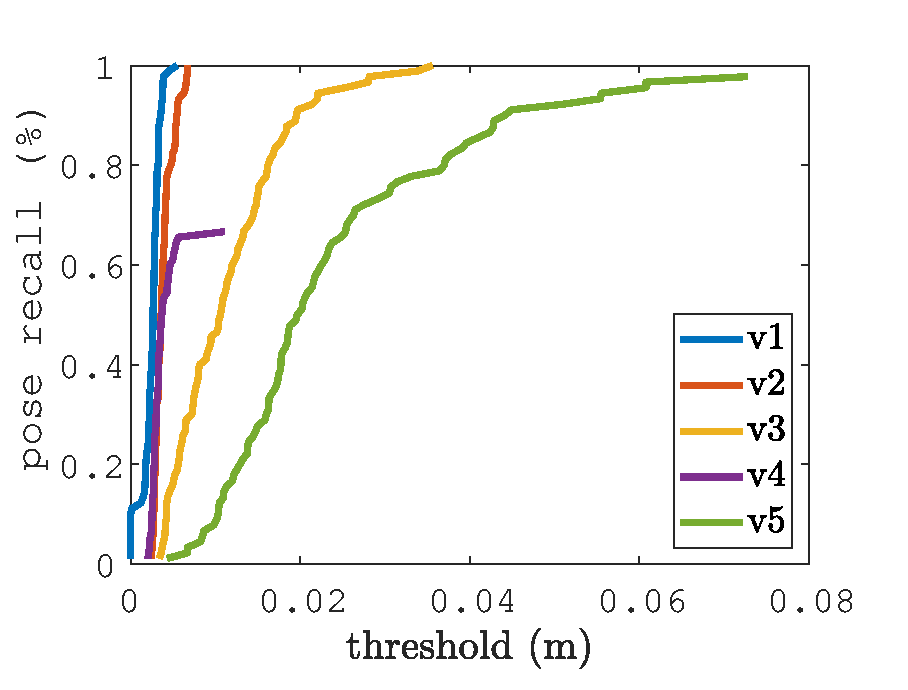
\includegraphics[height=2in]{Figures/real.eps}
\vspace{-0.1in}
\caption{(\textit{Left}): the blue bar represents the fraction of successful object transfers, the orange bar represents the percentage of unoccupied volume within the ideal target placement volume.(\textit{Middle:})\commentadd{the blue bar represents the average number of correction actions happened per experiment, the green bar represents the average number of toppling actions happened per experiment.}  (\textit{Right:}) The pose recall percentage over different thresholds is shown for the pipeline versions.
}
% \vspace{-0.2in}
\label{fig:real_data}
\end{figure*}

For consistency, an identical version of the problem is tested, with ``dove soap bars'' that are randomly thrown into the source bin $\binit$, which is placed on one side of the robot's reachable workspace (Fig \ref{fig:new_setup}). Only top-down grasps are allowed within a given alignment threshold. The start arrangement $\ainit$ of objects is intended to reflect a random pile, with $10$ repetitions of each experimental condition. The target bin $\btarget$ contains a $3\times 3$ grid arrangement of $9$ objects, on the same plane, with the stable face of the object targeted for placement. The complete pipeline uses a) corrective actions for fine adjustments, b) push-to-place actions for robust placement, c) toppling actions for increasing successes, and d) pose estimation for adjusting the object. The improvements introduced by these strategies are evaluated through the following comparison points, within the context of the proposed pipeline: 

\noindent \textbf{V1 - \commentadd{Full pipeline}}: The complete pipeline with all the primitives achieves the highest accuracy and success rate.

\noindent \textbf{V2 - No corrective actions}: The experiment corresponds to the use of \textbf{V1} without the fine correction module of Fig. \ref{fig:finer_fix}.

\noindent \textbf{V3 - No push-to-place actions}: This version is \textbf{V2} without the use of the robust placement module (Fig. \ref{fig:adaptive-pushing}) that performs push actions to achieve robust placement.

\noindent  \textbf{V4 - No toppling actions}: These experiments used \textbf{V2} without considering toppling actions to deal with objects not exposing a valid top surface that allows the target placement. 

\noindent  \textbf{V5 - (Baseline) No push-to-place, toppling, pose-estimation}: The naive baseline that solely uses a pose-unaware grasping module that reports locally graspable points and drops the grasped object at an end-effector pose raised from the center of the desired object position, with no adjustment in orientation. 

The metrics evaluated include the fraction of successful object transfers that succeed in moving objects to the target bin. The accuracy is captured in the threshold mentioned in Eq.~\eqref{eq:satisfaction} that is expressed in terms of a percentage of unoccupied volume within the ideal target placement volume. This was measured with a voxel discretization sufficient to elucidate the difference between the methods. The average data recorded is reported in Fig.~\ref{fig:final_bin_configs}. This error measure is proportional to the accuracy. The points to note for every version are detailed as follows.

%\begin{table}[]
%\centering
%\begin{tabular}{rlllll}
%\multicolumn{1}{l}{}                  & \textbf{V1}               & \textbf{V2}               & \textbf{V3}                & \textbf{V4}               & \textbf{V5}                \\ \cline{2-6} 
%\multicolumn{1}{r|}{\textbf{Success}} & \multicolumn{1}{l|}{1}    & \multicolumn{1}{l|}{1}    & \multicolumn{1}{l|}{1}     & \multicolumn{1}{l|}{0.67} & \multicolumn{1}{l|}{1}     \\ \cline{2-6} 
%\multicolumn{1}{r|}{\textbf{Error}}   & \multicolumn{1}{l|}{0.04} & \multicolumn{1}{l|}{0.87} & \multicolumn{1}{l|}{25.21} & \multicolumn{1}{l|}{31.40}    & \multicolumn{1}{l|}{49.55} \\ \cline{2-6} 
%\end{tabular}
%\label{table:success_accuracy}
%\caption{The successful object transfers and the error measure over $10$ runs of the different versions of the pipeline, packing $9$ objects per experiment.}
%\end{table}



The low error for \textbf{V1} corroborates the final bin placement evidence. On average $7$  corrective actions per experiment were invoked to achieve the high degree of accuracy.

The accuracy improvement obtained from corrective actions is evaluated in \textbf{V2}. While this version succeeded in dropping all the objects close to the correct target poses, application use-cases where a higher degree of accuracy is desired motivate the use of corrective actions. The integration of the corrective actions was done with higher error threshold during intermediate steps, and a much finer one for the final adjustment. Errors can typically arise from execution failure and pose misalignments. The less accurate these underlying processes are, the more important corrective actions become. 

\textbf{V3} only performs adjustments using pose estimation, and toppling. While, this is sufficient to successfully transfer all the objects, any difference of accuracy to \textbf{V2} would be introduced by the lack of push-to-place actions. Here there is complete reliance on the exactness of the execution and pose adjustments. Due to the proximity of adjacent object surfaces in the target grid arrangement, even minor errors get aggravated. However, due to the ability to reason about toppling, all the objects can be transferred to the target bin, even with this low accuracy. This is demonstrated in the occurrence of the failure to transfer all the objects. 

In \textbf{V4} any object that does not expose an permitted picking surface that makes the prehensile placement possible, is not picked. Any instance of the source bin, which ends with no such objects results in no valid picking actions that can make the approach proceed, and a failure is declared. The current behavior of \textbf{V4} drops the object if it is mistakenly grasped from the wrong surface. This can itself be used as a naive toppling primitive. It is important to note that there might be other alternative strategies that can deal with this failure, but the intent of this comparison is to demonstrate the importance of having a deliberate toppling strategy in the pipeline, that can change the object's orientation in the context of random starting arrangements of the object.  On average, over \textbf{V1, V2,} and \textbf{V3} the toppling primitive was required $4$ times per experiment. This highlights the necessity of this reasoning. Deliberate toppling however requires at least one additional pick action. The number of pick attempts per successful object transfer was $2.56$ for \textbf{V4}, whereas, in \textbf{V2} the same was $1.98$. This indicates that toppling is indeed necessary both in terms of success and efficiency of actions.  

Expectedly, \textbf{V5} has the lowest accuracy. However, since there is no reasoning about the pick surface, every object was transfered to the space of the bin. This has no guarantee to work if the object is larger. This drives the motivation for using a set of robust primitives for the packing problem.

Overall, the time for the experiments show a trend of increasing with the increasing complexity of the pipeline. The trade-off of accuracy versus time persists. On average, \textbf{V1} ran for $945$s while \textbf{V5} ran for $323$s.

% \begin{wrapfigure}[13]{r}{1in}
% \vspace*{-6mm}
%   \begin{center}
%   \includegraphics[width=1in,height=0.8in]{Figures/toothpaste.png}
% %  \smallskip\par
% \vspace{0.001in}
%   \includegraphics[width=1in, height=0.8in]{Figures/two_layer.PNG}
%   \end{center}
% \vspace*{-4mm}
%   \caption{Result for toothpaste and two-layer packing}
% \end{wrapfigure}


\subsection{Real-world Demonstrations}

Various demonstrative packing tasks (Fig~\ref{fig:final_bin_configs} \textit{bottom}) were executed to showcase the versatility of the proposed pipeline.

\noindent\textbf{Multi-layer packing}: With a sufficiently tall bin, objects can be packed in multiple layers. Running the method beyond the first plane of the grid effectively shifts all the operations to the higher plane. This is demonstrated in a standalone run.

\noindent\textbf{Different objects}: To validate the applicability of the method to other cuboidal objects, \textbf{V1} was performed for toothpastes. Over $5$ experiments,  with $4$ objects, every run succeeded in placing the object inside the bin.

\noindent\textbf{Heterogenous pile}: The source bin was filled up with two different kinds of objects and the pipeline was executed for each object sequentially, i.e., pack the \textit{toothpaste} first, and then the \textit{soap}, into two separate containers. The method is correctly capable of retrieving, and packing the desired objects from such a heterogeneous pile.

\noindent\textbf{Narrow-face reorientation}: The packing orientation is tested with the narrow (unstable) face of the cuboid being the contact surface. In such situations toppling has to reorient the object from its more stable wider face to the desired narrow face. 

\noindent\textbf{No-clearance Packing}: The target bin is resized to be of the exact dimensions as the cross section of the target arrangement. This leaves no clearance for the object for placements along the edges and corners of the $3\times 3$ grid. The compliance of the end-effector, and walls of the container are leveraged in the extended variant of the adaptive pushing primitive, to allow successful application of the proposed pipeline in this setting.

\rahul{


\subsection{Simulation: Adaptive Pushing}

\begin{figure*}[ht]
    \centering
    \begin{overpic}[height=1.4in]{Figures/vol_err_plot.png}%
    \put(450,-50){(a)}%
    \end{overpic}
    % \includegraphics[height=1.4in]{Figures/vol_err_plot.png}
    \begin{overpic}[height=1.55in]{Figures/expansion_higher_noise.eps}%
    \put(450,-50){(b)}%
    \end{overpic}
    % 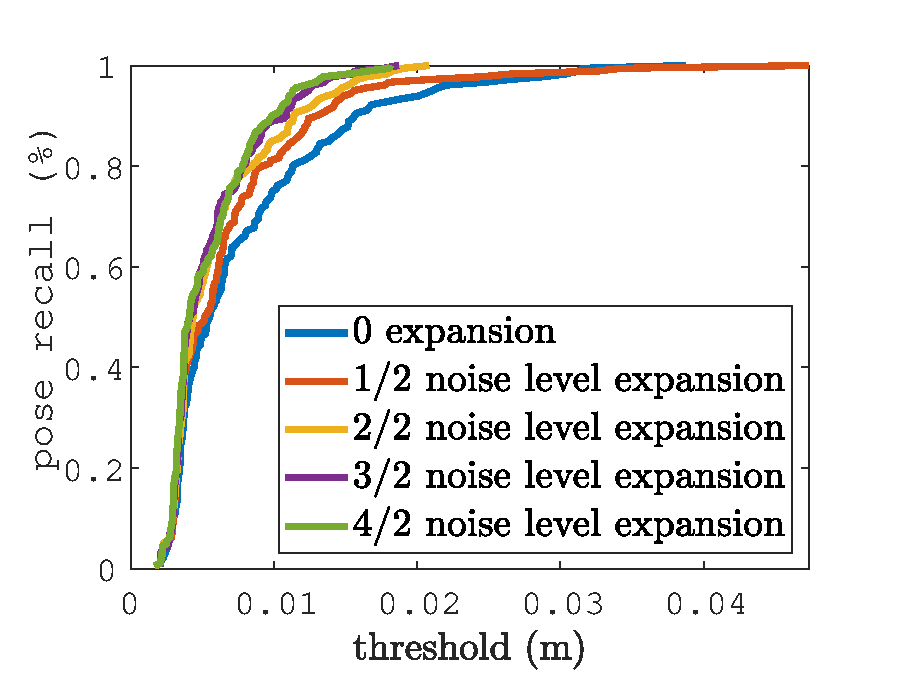
\includegraphics[height=1.55in]{Figures/expansion_higher_noise.eps}
    \begin{overpic}[height=1.55in]{Figures/z_lift_higher_noise.eps}%
    \put(450,-50){(c)}%
    \end{overpic}   
    % 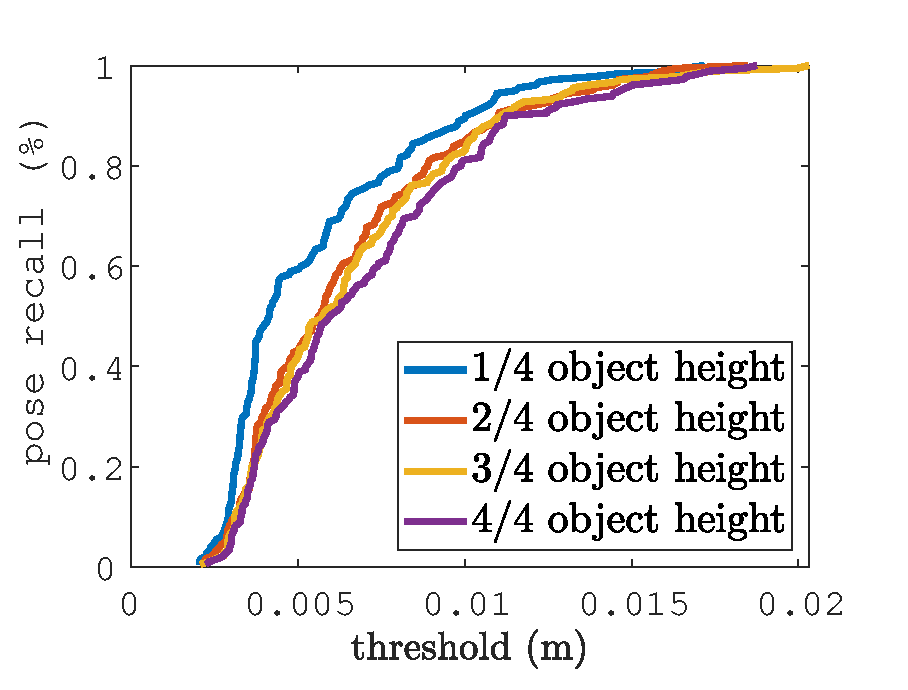
\includegraphics[height=1.55in]{Figures/z_lift_higher_noise.eps}
    \caption{(\textit{a}) Volumetric error of proposed adaptive pushing primitive compared with baseline method under two noise levels. Pushing distance is a parameter for the baseline method. 
    Pose recall against the parameter for adaptive pushing. \textit{b} expansion size of object model, \textit{(c)} height of pre-push pose
    }
    \label{fig:adaptive-pushing-compare}
\end{figure*}

To examine the effectiveness of proposed adaptive pushing primitive on reducing the packing error, experiments were executed to compare proposed method with a simple baseline method. For each new object to place, given the target pose, the baseline method will calculate a pre-push pose using a fixed displacement. During the simulation, uniform random noise is applied to the pre-push pose in both translation and rotation direction, to evaluate the performance under different level of noise, two noise levels are introduced. The lower noise level applies 1 cm deviation to the translation direction and 5 degrees deviation to the rotation direction, while the higher noise level applies 2 cm deviation and 15 degrees accordingly. 
In the experiment, the proposed method is compared against the baseline method with different fixed displacement as parameters. The result is shown in Fig \ref{fig:adaptive-pushing-compare}. From the result, we can observe that as the pushing distance decreases for the baseline method, its performance becomes worse compared with the proposed adaptive primitive. When the pushing distance is larger than 5cm, the baseline method's performance is better than the adaptive primitive, but large fixed pushing distance will also cause issues in restricted space such as in the packing scenario. 
% \begin{figure}
%     \centering
%     \includegraphics[width=0.5\textwidth]{Figures/vol_err_plot.png}
%     \caption{Volumetric error of proposed adaptive pushing primitive compared with baseline method under two noise levels. Pushing distance is a parameter for the baseline method. }
%     \label{fig:adaptive-pushing-compare}
% \end{figure}

% \begin{figure}
%     \centering
%     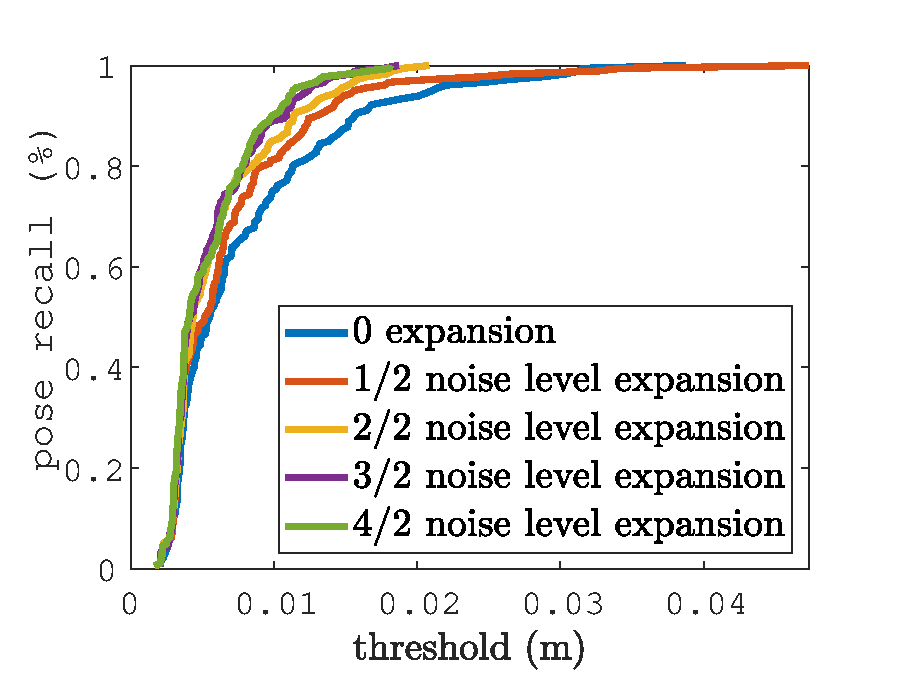
\includegraphics[width=0.49\linewidth]{Figures/expansion_higher_noise.eps}
%     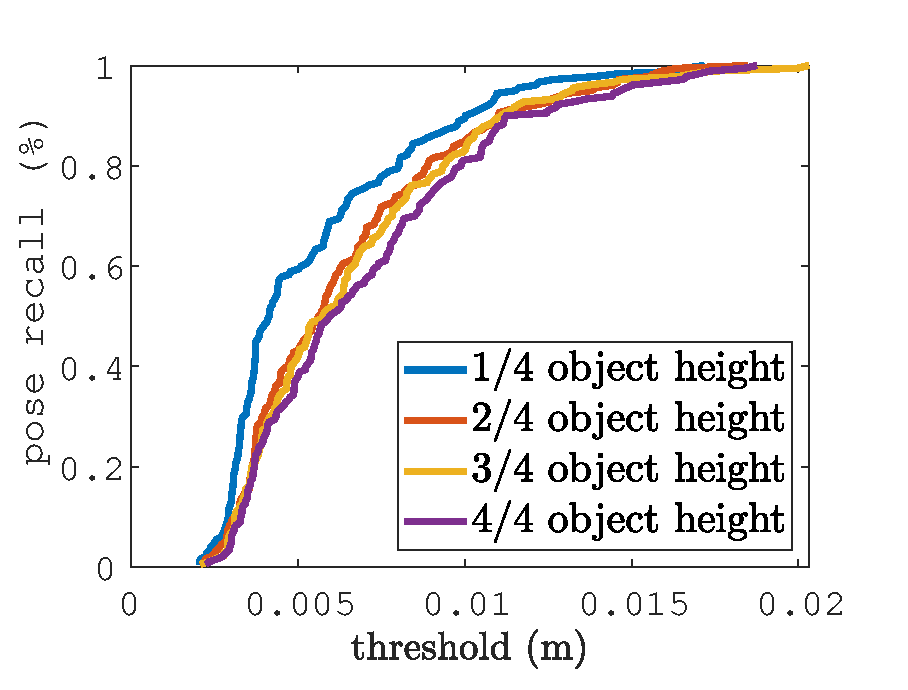
\includegraphics[width=0.49\linewidth]{Figures/z_lift_higher_noise.eps}
%     \caption{Pose recall against the parameter for adaptive pushing. (left) expansion size of object model, (right) height of pre-push pose}
%     \label{fig:expansion_simulation}
% \end{figure}




To further evaluate the adaptive pushing primitive, we have examined the influence of two parameters. The first is the expansion size of object model for collision checking, the second factor is the height of pre-push pose. The evaluation will help to determine a best strategy for choosing these parameters and also validate our understanding of proposed primitive. The result is shown in Fig \ref{fig:adaptive-pushing-compare}, two figures are corresponding to the mentioned two parameters. For the expansion size, we tested different expansions relative to the noise level and check how the pose recall changes according to the expansion sizes.  The result under higher noise is shown in the left figure, we can observe that once the expansion size drops below the noise level, the pose recall curve drops rapidly. Another observation is that the pose recall is much more sensitive to expansion size under higher noise level. Under the lower noise level, the pose recall curves are much closer to each other compared under higher noise level. At last, in order to achieve stable performance, it is best to choose expansion size that is bigger than 2 times of the noise level. 
% \begin{figure}
%     \centering
%     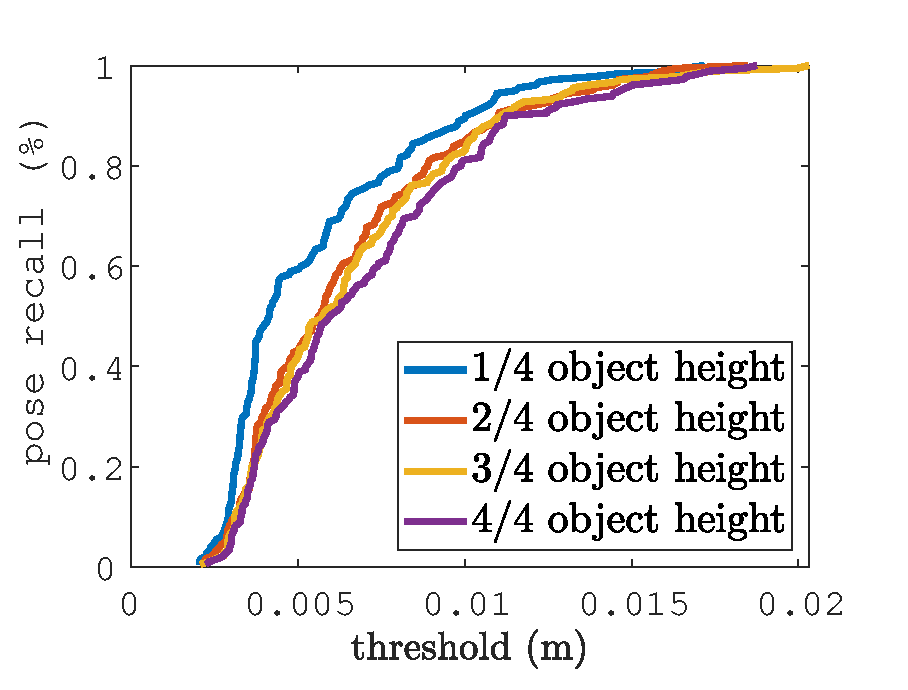
\includegraphics[width=0.49\linewidth]{Figures/z_lift_higher_noise.eps}%
%     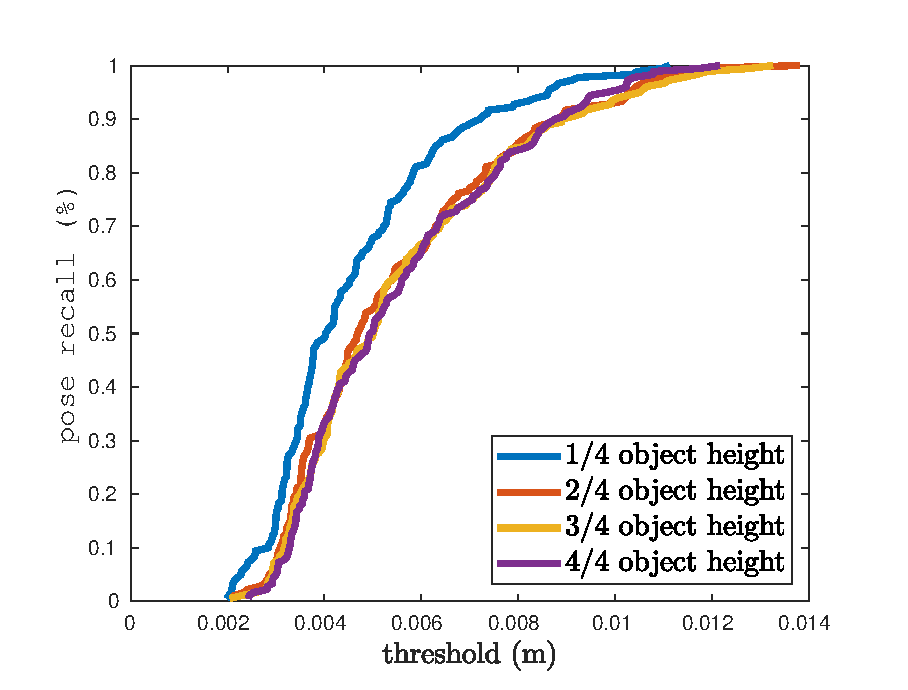
\includegraphics[width=0.49\linewidth]{Figures/z_lift_lower_noise.eps}
%     \caption{Pose recall against the height of pre-push pose}
%     \label{fig:height_pre_push_pose_simulation}
% \end{figure}
For the height of the pre-push pose, we tested different value relative to the object's height and check how the pose recall changes accordingly. The result is shown in the right figure of Fig \ref{fig:adaptive-pushing-compare}. From the figure, we can observe that the pose recall curve drops rapidly after the height of pre-push pose increases over 1/4 of object height under both noise levels. 

}

\changkyu{

\subsection{Simulation: Fine Correction}

\begin{figure*}[ht]
    \centering
    \includegraphics[width=0.34\textwidth,valign=t]{./Figures/res_recall.png}
    \includegraphics[width=0.64\textwidth,valign=t]{./Figures/res_step.png}
    \caption{Pose recall (left) and volumetric error (ADI) against the number of placed objects (right) with and without the fine correction module under different noise levels.}
    \label{fig:res_recall}
\end{figure*}

We evaluated the fine correction module on the same simulation setup with the same noise levels: 1cm deviation to the translation and 5 degrees deviation to the rotation, 2cm and 15 degrees deviations accordingly.
We compared \textbf{V1 - Full Pipeline} that has the all the primitives including the fine correction module and \textbf{V2 - No corrective actions} that uses \textbf{V1} but has no fine correction module.
The fine correction is repeated until the point cloud is aligned with the desired goal poses given a threshold $\epsilon=0.5cm$, but it is never repeated more than $4$ times for each placement.

Fig~\ref{fig:res_recall} (left) shows the pose recall rate under different noise levels.
In this experiment, $1.03 (\pm0.80)$ number of corrective actions are executed per placement in average.
Without the corrective module (\textbf{V2}), the pose recall curve dropped as the noise level raised.
However, the full pipeline \textbf{V1} kept a high recall rate regardless of the noises.
Fig~\ref{fig:res_recall} (right) shows the volumetric error (ADI) against the number of placed objects.
Whenever the fine correction module was executed, the volumetric error dropped under its threshold (\textbf{V1}), while the error of \textbf{V2} does not decrease dramatically.
The fine correction module not only corrected the misplacement due to the simulated noise, but also it prevents the situation that the misaligned objects affect to the future placement.

}
% Contributions of the paper we want to demonstrate and improvements relative to current version:

%  - Picking so as to expose the right surface: improve the dropping so that we reason how to reorient it but treating the original bin as a terrain

% - robust placement at the target bin: we should pick automatically the placement of the object and the direction of the pushing operation by taking into account the interaction of multiple objects (i.e., with the placement of the last object fix the orientation of the previous ones as well)

% - toppling and pushing fix: use the same reasoning about the interaction of multiple objects 

% Comparison Experiment, One 3x3 layer (without foam):

% A. Base case - without pose estimation, find a flat surface in the source and drop it in a pre-defined location (drop from higher distance)
 
% B. With pose estimation, prioritizing flat surface, trust the original pose estimation, you go directly at the target configuration but drop from a height

% C. Same as before but verifying at the source bin: with dropping the object when we detect that we picked the wrong surface

% D. Same as before but verifying at the target bin: pushing operation - first time we place at the bottom of the bin

% E. Same as before but we also evaluate success from vision and perform toppling and pushing operations directly from data so as to maintain an invariant of packed objects

% Demonstrations: 

%  - different object: the toothpastes
 
%  - multiple layers (without the foam)
 
%  - with the foam 

% Metrics?

%  - percent of boxes transported into the target bin
 
%  - distance from preferred pose (intersection over union)
 
%  - time
 
%  - \# of grasps, \# of times we topple (and how many times we succeeded), \# of times we fix the placement of objects (and how many times we succeeded) 

% Save the videos for all the experiments in a URL

% Bring up in the discussion section of the paper the following future work points: 

%  - what if the side you need to pick it up is the unstable one?
 
%  - perform the robust placement in SE(2) instead of R(2)

% - topple directly objects if there is no good surface exposed

% - the location of the bin may not be known

% - we want to eventually place object of different types in 
%  the same bin

\section{Discussion}
\label{section:discussion}
The proposed pipeline indicates intriguing nuances of the packing problem. The use of a minimal, suction-based end-effector is a cost-effective, simple and relatively robust way to pick objects but does not easily allow for complex grasp reasoning, regrasping, or within-hand manipulation. The proposed pipeline achieves high accuracy by leveraging the compliance of the suction cup and the environment, while the object is attached. It uses robust reasoning to incrementally correct errors, instead of compounding them. While it can be argued that better baseline components can be developed to minimize uncertainty, the overall philosophy of robust, minimal, and compliant reasoning remains unchanged. 

The proposed system and primitives can also deal with cubic objects with different sizes and can be extended to non-cubic objects by adapting the object models. The key adaptation corresponds to identifying an appropriate packing arrangement $\atarget$ (potentially labeled in this case) in the target bin and the corresponding picking order from the initial bin. Future work will also explore speeding up performance and dealing with algorithmic challenges: the combinatorial reasoning over possible placements, physics-based reasoning to further improve pushing and toppling, as well as extending to more adaptive end-effectors. The platform can also be utilized as a training testbed for reinforcement learning to automatically discover robust primitives for solving packing tasks.

%https://preview.overleaf.com/public/vygnpnpqtbct/images/6836fea5b56bab9aa94fc612378769a9aaa648b9.jpeg

\bibliographystyle{Bibliography/IEEEtran}
\bibliography{Bibliography/manip}

\end{document}
